\documentclass[journal]{IEEEtran}
\usepackage{fontspec}
\setmainfont{TeX Gyre Termes}
\usepackage{amsmath,amssymb,bm}
\usepackage{graphicx}
\usepackage{booktabs,multirow,array}
\newcolumntype{L}[1]{>{\raggedright\arraybackslash}p{#1}}
\usepackage{algorithm}
\usepackage[noend]{algpseudocode}
\usepackage{url}
\usepackage[hidelinks]{hyperref}
\renewcommand{\IEEEkeywordsname}{Từ khóa}
\renewcommand{\abstractname}{Tóm tắt}
\renewcommand{\tablename}{BẢNG}
\renewcommand{\figurename}{Hình}
\renewcommand{\refname}{Tài liệu tham khảo}
\renewcommand{\appendixname}{Phụ lục}
\renewcommand{\IEEEproofname}{Chứng minh}
\floatname{algorithm}{Thuật toán}
\algrenewcommand\algorithmicrequire{\textbf{Đầu vào:}}
\algrenewcommand\algorithmicensure{\textbf{Đầu ra:}}
\algrenewcommand\algorithmicfor{\textbf{for}}
\algrenewcommand\algorithmicdo{\textbf{do}}
\newtheorem{definition}{Định nghĩa}
\newtheorem{proposition}{Mệnh đề}
\newtheorem{lemma}{Bổ đề}
\newtheorem{remark}{Nhận xét}
\newcommand{\code}[1]{\texttt{#1}}
\newcommand{\HVadj}{\mathrm{HV}_{\text{adj}}}
% generated by build_report.py from runs/ — do not edit
\newcommand{\R}[1]{\ifcsname R@#1\endcsname\csname R@#1\endcsname\else\errmessage{No number for key #1}\fi}
\expandafter\def\csname R@L1-dauc-fold\endcsname{0,0033}
\expandafter\def\csname R@L1-dauc-global\endcsname{0,0041}
\expandafter\def\csname R@S1-ipa-cox\endcsname{0,155}
\expandafter\def\csname R@S1-ipa-interval\endcsname{0,284}
\expandafter\def\csname R@S1-oe-cox\endcsname{1,83}
\expandafter\def\csname R@S1-oe-interval\endcsname{1,00}
\expandafter\def\csname R@S2b-auc-ci\endcsname{(−0,007; 0,034)}
\expandafter\def\csname R@S2b-bsi-dauc\endcsname{0,006}
\expandafter\def\csname R@S2b-dauc\endcsname{0,012}
\expandafter\def\csname R@S2b-persons\endcsname{235}
\expandafter\def\csname R@S8-1-dauc\endcsname{0,002}
\expandafter\def\csname R@S8-1-persons\endcsname{508}
\expandafter\def\csname R@S8-30-dauc\endcsname{0,002}
\expandafter\def\csname R@S8-30-persons\endcsname{318}
\expandafter\def\csname R@S8-7-dauc\endcsname{0,002}
\expandafter\def\csname R@S8-7-persons\endcsname{441}
\expandafter\def\csname R@S9-auc-older\endcsname{0,899}
\expandafter\def\csname R@S9-auc-recent\endcsname{0,891}
\expandafter\def\csname R@available-persons-M0\endcsname{865}
\expandafter\def\csname R@available-persons-M1\endcsname{811}
\expandafter\def\csname R@available-persons-M2\endcsname{604}
\expandafter\def\csname R@available-persons-M3\endcsname{558}
\expandafter\def\csname R@cm-cv-M0-15-f1\endcsname{0,60}
\expandafter\def\csname R@cm-cv-M0-15-flagged\endcsname{0,73}
\expandafter\def\csname R@cm-cv-M0-15-npv\endcsname{0,97}
\expandafter\def\csname R@cm-cv-M0-15-ppv\endcsname{0,44}
\expandafter\def\csname R@cm-cv-M0-15-sensitivity\endcsname{0,97}
\expandafter\def\csname R@cm-cv-M0-15-specificity\endcsname{0,39}
\expandafter\def\csname R@cm-cv-M0-30-f1\endcsname{0,74}
\expandafter\def\csname R@cm-cv-M0-30-flagged\endcsname{0,38}
\expandafter\def\csname R@cm-cv-M0-30-npv\endcsname{0,89}
\expandafter\def\csname R@cm-cv-M0-30-ppv\endcsname{0,69}
\expandafter\def\csname R@cm-cv-M0-30-sensitivity\endcsname{0,80}
\expandafter\def\csname R@cm-cv-M0-30-specificity\endcsname{0,82}
\expandafter\def\csname R@cm-cv-M1-15-f1\endcsname{0,63}
\expandafter\def\csname R@cm-cv-M1-15-flagged\endcsname{0,68}
\expandafter\def\csname R@cm-cv-M1-15-npv\endcsname{0,96}
\expandafter\def\csname R@cm-cv-M1-15-ppv\endcsname{0,46}
\expandafter\def\csname R@cm-cv-M1-15-sensitivity\endcsname{0,97}
\expandafter\def\csname R@cm-cv-M1-15-specificity\endcsname{0,46}
\expandafter\def\csname R@cm-cv-M1-30-f1\endcsname{0,74}
\expandafter\def\csname R@cm-cv-M1-30-flagged\endcsname{0,37}
\expandafter\def\csname R@cm-cv-M1-30-npv\endcsname{0,89}
\expandafter\def\csname R@cm-cv-M1-30-ppv\endcsname{0,70}
\expandafter\def\csname R@cm-cv-M1-30-sensitivity\endcsname{0,79}
\expandafter\def\csname R@cm-cv-M1-30-specificity\endcsname{0,83}
\expandafter\def\csname R@cm-cv-M2-15-f1\endcsname{0,62}
\expandafter\def\csname R@cm-cv-M2-15-flagged\endcsname{0,69}
\expandafter\def\csname R@cm-cv-M2-15-npv\endcsname{0,96}
\expandafter\def\csname R@cm-cv-M2-15-ppv\endcsname{0,46}
\expandafter\def\csname R@cm-cv-M2-15-sensitivity\endcsname{0,96}
\expandafter\def\csname R@cm-cv-M2-15-specificity\endcsname{0,45}
\expandafter\def\csname R@cm-cv-M2-30-f1\endcsname{0,75}
\expandafter\def\csname R@cm-cv-M2-30-flagged\endcsname{0,38}
\expandafter\def\csname R@cm-cv-M2-30-npv\endcsname{0,90}
\expandafter\def\csname R@cm-cv-M2-30-ppv\endcsname{0,70}
\expandafter\def\csname R@cm-cv-M2-30-sensitivity\endcsname{0,80}
\expandafter\def\csname R@cm-cv-M2-30-specificity\endcsname{0,83}
\expandafter\def\csname R@cm-cv-M3-15-f1\endcsname{0,63}
\expandafter\def\csname R@cm-cv-M3-15-flagged\endcsname{0,68}
\expandafter\def\csname R@cm-cv-M3-15-npv\endcsname{0,96}
\expandafter\def\csname R@cm-cv-M3-15-ppv\endcsname{0,47}
\expandafter\def\csname R@cm-cv-M3-15-sensitivity\endcsname{0,96}
\expandafter\def\csname R@cm-cv-M3-15-specificity\endcsname{0,46}
\expandafter\def\csname R@cm-cv-M3-30-f1\endcsname{0,76}
\expandafter\def\csname R@cm-cv-M3-30-flagged\endcsname{0,37}
\expandafter\def\csname R@cm-cv-M3-30-npv\endcsname{0,90}
\expandafter\def\csname R@cm-cv-M3-30-ppv\endcsname{0,71}
\expandafter\def\csname R@cm-cv-M3-30-sensitivity\endcsname{0,81}
\expandafter\def\csname R@cm-cv-M3-30-specificity\endcsname{0,84}
\expandafter\def\csname R@cm-test-M0-15-f1\endcsname{0,66}
\expandafter\def\csname R@cm-test-M0-15-flagged\endcsname{0,72}
\expandafter\def\csname R@cm-test-M0-15-npv\endcsname{0,98}
\expandafter\def\csname R@cm-test-M0-15-ppv\endcsname{0,49}
\expandafter\def\csname R@cm-test-M0-15-sensitivity\endcsname{0,98}
\expandafter\def\csname R@cm-test-M0-15-specificity\endcsname{0,43}
\expandafter\def\csname R@cm-test-M0-30-f1\endcsname{0,79}
\expandafter\def\csname R@cm-test-M0-30-flagged\endcsname{0,41}
\expandafter\def\csname R@cm-test-M0-30-npv\endcsname{0,90}
\expandafter\def\csname R@cm-test-M0-30-ppv\endcsname{0,74}
\expandafter\def\csname R@cm-test-M0-30-sensitivity\endcsname{0,84}
\expandafter\def\csname R@cm-test-M0-30-specificity\endcsname{0,83}
\expandafter\def\csname R@cm-test-M1-15-f1\endcsname{0,72}
\expandafter\def\csname R@cm-test-M1-15-flagged\endcsname{0,63}
\expandafter\def\csname R@cm-test-M1-15-npv\endcsname{1,00}
\expandafter\def\csname R@cm-test-M1-15-ppv\endcsname{0,57}
\expandafter\def\csname R@cm-test-M1-15-sensitivity\endcsname{1,00}
\expandafter\def\csname R@cm-test-M1-15-specificity\endcsname{0,57}
\expandafter\def\csname R@cm-test-M1-30-f1\endcsname{0,81}
\expandafter\def\csname R@cm-test-M1-30-flagged\endcsname{0,41}
\expandafter\def\csname R@cm-test-M1-30-npv\endcsname{0,92}
\expandafter\def\csname R@cm-test-M1-30-ppv\endcsname{0,76}
\expandafter\def\csname R@cm-test-M1-30-sensitivity\endcsname{0,86}
\expandafter\def\csname R@cm-test-M1-30-specificity\endcsname{0,85}
\expandafter\def\csname R@cm-test-M2-15-f1\endcsname{0,73}
\expandafter\def\csname R@cm-test-M2-15-flagged\endcsname{0,60}
\expandafter\def\csname R@cm-test-M2-15-npv\endcsname{0,98}
\expandafter\def\csname R@cm-test-M2-15-ppv\endcsname{0,58}
\expandafter\def\csname R@cm-test-M2-15-sensitivity\endcsname{0,98}
\expandafter\def\csname R@cm-test-M2-15-specificity\endcsname{0,61}
\expandafter\def\csname R@cm-test-M2-30-f1\endcsname{0,79}
\expandafter\def\csname R@cm-test-M2-30-flagged\endcsname{0,39}
\expandafter\def\csname R@cm-test-M2-30-npv\endcsname{0,90}
\expandafter\def\csname R@cm-test-M2-30-ppv\endcsname{0,76}
\expandafter\def\csname R@cm-test-M2-30-sensitivity\endcsname{0,83}
\expandafter\def\csname R@cm-test-M2-30-specificity\endcsname{0,85}
\expandafter\def\csname R@cm-test-M3-15-f1\endcsname{0,69}
\expandafter\def\csname R@cm-test-M3-15-flagged\endcsname{0,68}
\expandafter\def\csname R@cm-test-M3-15-npv\endcsname{1,00}
\expandafter\def\csname R@cm-test-M3-15-ppv\endcsname{0,53}
\expandafter\def\csname R@cm-test-M3-15-sensitivity\endcsname{1,00}
\expandafter\def\csname R@cm-test-M3-15-specificity\endcsname{0,51}
\expandafter\def\csname R@cm-test-M3-30-f1\endcsname{0,79}
\expandafter\def\csname R@cm-test-M3-30-flagged\endcsname{0,40}
\expandafter\def\csname R@cm-test-M3-30-npv\endcsname{0,90}
\expandafter\def\csname R@cm-test-M3-30-ppv\endcsname{0,74}
\expandafter\def\csname R@cm-test-M3-30-sensitivity\endcsname{0,84}
\expandafter\def\csname R@cm-test-M3-30-specificity\endcsname{0,84}
\expandafter\def\csname R@cv-M0-1095-auc\endcsname{0,874}
\expandafter\def\csname R@cv-M0-1095-brier\endcsname{0,155}
\expandafter\def\csname R@cv-M0-1095-ipa\endcsname{0,382}
\expandafter\def\csname R@cv-M0-1095-nb20\endcsname{0,299}
\expandafter\def\csname R@cv-M0-1095-oe\endcsname{0,93}
\expandafter\def\csname R@cv-M0-1095-slope\endcsname{1,79}
\expandafter\def\csname R@cv-M0-365-auc\endcsname{0,866}
\expandafter\def\csname R@cv-M0-365-brier\endcsname{0,136}
\expandafter\def\csname R@cv-M0-365-ipa\endcsname{0,259}
\expandafter\def\csname R@cv-M0-365-nb20\endcsname{0,148}
\expandafter\def\csname R@cv-M0-365-oe\endcsname{1,01}
\expandafter\def\csname R@cv-M0-365-slope\endcsname{1,77}
\expandafter\def\csname R@cv-M0-730-auc\endcsname{0,876}
\expandafter\def\csname R@cv-M0-730-brier\endcsname{0,149}
\expandafter\def\csname R@cv-M0-730-ipa\endcsname{0,340}
\expandafter\def\csname R@cv-M0-730-nb20\endcsname{0,231}
\expandafter\def\csname R@cv-M0-730-oe\endcsname{0,96}
\expandafter\def\csname R@cv-M0-730-slope\endcsname{1,67}
\expandafter\def\csname R@cv-M1-1095-auc\endcsname{0,886}
\expandafter\def\csname R@cv-M1-1095-brier\endcsname{0,145}
\expandafter\def\csname R@cv-M1-1095-ipa\endcsname{0,419}
\expandafter\def\csname R@cv-M1-1095-nb20\endcsname{0,306}
\expandafter\def\csname R@cv-M1-1095-oe\endcsname{0,92}
\expandafter\def\csname R@cv-M1-1095-slope\endcsname{1,75}
\expandafter\def\csname R@cv-M1-365-auc\endcsname{0,868}
\expandafter\def\csname R@cv-M1-365-brier\endcsname{0,134}
\expandafter\def\csname R@cv-M1-365-ipa\endcsname{0,269}
\expandafter\def\csname R@cv-M1-365-nb20\endcsname{0,149}
\expandafter\def\csname R@cv-M1-365-oe\endcsname{1,00}
\expandafter\def\csname R@cv-M1-365-slope\endcsname{1,68}
\expandafter\def\csname R@cv-M1-730-auc\endcsname{0,886}
\expandafter\def\csname R@cv-M1-730-brier\endcsname{0,142}
\expandafter\def\csname R@cv-M1-730-ipa\endcsname{0,371}
\expandafter\def\csname R@cv-M1-730-nb20\endcsname{0,244}
\expandafter\def\csname R@cv-M1-730-oe\endcsname{0,96}
\expandafter\def\csname R@cv-M1-730-slope\endcsname{1,60}
\expandafter\def\csname R@cv-M1M0-1095-auc-ci\endcsname{(−0,008; 0,033)}
\expandafter\def\csname R@cv-M1M0-1095-dauc\endcsname{0,012}
\expandafter\def\csname R@cv-M1M0-1095-dnb\endcsname{0,011}
\expandafter\def\csname R@cv-M1M0-1095-nb-ci\endcsname{(0,000; 0,023)}
\expandafter\def\csname R@cv-M1M0-1095-rule\endcsname{Bất định}
\expandafter\def\csname R@cv-M1M0-1095-rule-lc\endcsname{bất định}
\expandafter\def\csname R@cv-M1M0-365-auc-ci\endcsname{(−0,018; 0,024)}
\expandafter\def\csname R@cv-M1M0-365-dauc\endcsname{0,002}
\expandafter\def\csname R@cv-M1M0-365-dnb\endcsname{0,005}
\expandafter\def\csname R@cv-M1M0-365-nb-ci\endcsname{(−0,006; 0,016)}
\expandafter\def\csname R@cv-M1M0-365-rule\endcsname{Bất định}
\expandafter\def\csname R@cv-M1M0-365-rule-lc\endcsname{bất định}
\expandafter\def\csname R@cv-M1M0-730-auc-ci\endcsname{(−0,011; 0,032)}
\expandafter\def\csname R@cv-M1M0-730-dauc\endcsname{0,010}
\expandafter\def\csname R@cv-M1M0-730-dnb\endcsname{0,007}
\expandafter\def\csname R@cv-M1M0-730-nb-ci\endcsname{(−0,007; 0,020)}
\expandafter\def\csname R@cv-M1M0-730-rule\endcsname{Bất định}
\expandafter\def\csname R@cv-M1M0-730-rule-lc\endcsname{bất định}
\expandafter\def\csname R@cv-M2-1095-auc\endcsname{0,889}
\expandafter\def\csname R@cv-M2-1095-brier\endcsname{0,145}
\expandafter\def\csname R@cv-M2-1095-ipa\endcsname{0,422}
\expandafter\def\csname R@cv-M2-1095-nb20\endcsname{0,305}
\expandafter\def\csname R@cv-M2-1095-oe\endcsname{0,92}
\expandafter\def\csname R@cv-M2-1095-slope\endcsname{1,83}
\expandafter\def\csname R@cv-M2-365-auc\endcsname{0,871}
\expandafter\def\csname R@cv-M2-365-brier\endcsname{0,134}
\expandafter\def\csname R@cv-M2-365-ipa\endcsname{0,272}
\expandafter\def\csname R@cv-M2-365-nb20\endcsname{0,149}
\expandafter\def\csname R@cv-M2-365-oe\endcsname{1,01}
\expandafter\def\csname R@cv-M2-365-slope\endcsname{1,72}
\expandafter\def\csname R@cv-M2-730-auc\endcsname{0,888}
\expandafter\def\csname R@cv-M2-730-brier\endcsname{0,141}
\expandafter\def\csname R@cv-M2-730-ipa\endcsname{0,374}
\expandafter\def\csname R@cv-M2-730-nb20\endcsname{0,243}
\expandafter\def\csname R@cv-M2-730-oe\endcsname{0,96}
\expandafter\def\csname R@cv-M2-730-slope\endcsname{1,65}
\expandafter\def\csname R@cv-M2M1-1095-auc-ci\endcsname{(−0,008; 0,013)}
\expandafter\def\csname R@cv-M2M1-1095-dauc\endcsname{0,003}
\expandafter\def\csname R@cv-M2M1-1095-dnb\endcsname{−0,001}
\expandafter\def\csname R@cv-M2M1-1095-nb-ci\endcsname{(−0,010; 0,006)}
\expandafter\def\csname R@cv-M2M1-1095-rule\endcsname{Tương đương}
\expandafter\def\csname R@cv-M2M1-1095-rule-lc\endcsname{tương đương}
\expandafter\def\csname R@cv-M2M1-365-auc-ci\endcsname{(−0,007; 0,011)}
\expandafter\def\csname R@cv-M2M1-365-dauc\endcsname{0,002}
\expandafter\def\csname R@cv-M2M1-365-dnb\endcsname{−0,002}
\expandafter\def\csname R@cv-M2M1-365-nb-ci\endcsname{(−0,008; 0,005)}
\expandafter\def\csname R@cv-M2M1-365-rule\endcsname{Tương đương}
\expandafter\def\csname R@cv-M2M1-365-rule-lc\endcsname{tương đương}
\expandafter\def\csname R@cv-M2M1-730-auc-ci\endcsname{(−0,007; 0,013)}
\expandafter\def\csname R@cv-M2M1-730-dauc\endcsname{0,002}
\expandafter\def\csname R@cv-M2M1-730-dnb\endcsname{0,000}
\expandafter\def\csname R@cv-M2M1-730-nb-ci\endcsname{(−0,005; 0,006)}
\expandafter\def\csname R@cv-M2M1-730-rule\endcsname{Tương đương}
\expandafter\def\csname R@cv-M2M1-730-rule-lc\endcsname{tương đương}
\expandafter\def\csname R@cv-M3-1095-auc\endcsname{0,892}
\expandafter\def\csname R@cv-M3-1095-brier\endcsname{0,142}
\expandafter\def\csname R@cv-M3-1095-ipa\endcsname{0,433}
\expandafter\def\csname R@cv-M3-1095-nb20\endcsname{0,306}
\expandafter\def\csname R@cv-M3-1095-oe\endcsname{0,91}
\expandafter\def\csname R@cv-M3-1095-slope\endcsname{1,82}
\expandafter\def\csname R@cv-M3-365-auc\endcsname{0,875}
\expandafter\def\csname R@cv-M3-365-brier\endcsname{0,132}
\expandafter\def\csname R@cv-M3-365-ipa\endcsname{0,279}
\expandafter\def\csname R@cv-M3-365-nb20\endcsname{0,155}
\expandafter\def\csname R@cv-M3-365-oe\endcsname{1,01}
\expandafter\def\csname R@cv-M3-365-slope\endcsname{1,68}
\expandafter\def\csname R@cv-M3-730-auc\endcsname{0,891}
\expandafter\def\csname R@cv-M3-730-brier\endcsname{0,139}
\expandafter\def\csname R@cv-M3-730-ipa\endcsname{0,384}
\expandafter\def\csname R@cv-M3-730-nb20\endcsname{0,243}
\expandafter\def\csname R@cv-M3-730-oe\endcsname{0,96}
\expandafter\def\csname R@cv-M3-730-slope\endcsname{1,57}
\expandafter\def\csname R@cv-M3M2-1095-auc-ci\endcsname{(−0,007; 0,013)}
\expandafter\def\csname R@cv-M3M2-1095-dauc\endcsname{0,003}
\expandafter\def\csname R@cv-M3M2-1095-dnb\endcsname{0,001}
\expandafter\def\csname R@cv-M3M2-1095-nb-ci\endcsname{(−0,006; 0,008)}
\expandafter\def\csname R@cv-M3M2-1095-rule\endcsname{Tương đương}
\expandafter\def\csname R@cv-M3M2-1095-rule-lc\endcsname{tương đương}
\expandafter\def\csname R@cv-M3M2-365-auc-ci\endcsname{(−0,003; 0,013)}
\expandafter\def\csname R@cv-M3M2-365-dauc\endcsname{0,005}
\expandafter\def\csname R@cv-M3M2-365-dnb\endcsname{0,004}
\expandafter\def\csname R@cv-M3M2-365-nb-ci\endcsname{(−0,003; 0,011)}
\expandafter\def\csname R@cv-M3M2-365-rule\endcsname{Bất định}
\expandafter\def\csname R@cv-M3M2-365-rule-lc\endcsname{bất định}
\expandafter\def\csname R@cv-M3M2-730-auc-ci\endcsname{(−0,006; 0,012)}
\expandafter\def\csname R@cv-M3M2-730-dauc\endcsname{0,003}
\expandafter\def\csname R@cv-M3M2-730-dnb\endcsname{0,002}
\expandafter\def\csname R@cv-M3M2-730-nb-ci\endcsname{(−0,005; 0,007)}
\expandafter\def\csname R@cv-M3M2-730-rule\endcsname{Tương đương}
\expandafter\def\csname R@cv-M3M2-730-rule-lc\endcsname{tương đương}
\expandafter\def\csname R@cv-auc-range\endcsname{0,866–0,892}
\expandafter\def\csname R@cv-design\endcsname{5 × 20}
\expandafter\def\csname R@cv-nb20-range\endcsname{0,231–0,244}
\expandafter\def\csname R@cv-observed-ipcw\endcsname{0,327}
\expandafter\def\csname R@cv-observed-turnbull\endcsname{0,287}
\expandafter\def\csname R@cv-oe-range\endcsname{0,91–1,01}
\expandafter\def\csname R@cv-per-group\endcsname{56}
\expandafter\def\csname R@cv-slope-range\endcsname{1,57–1,83}
\expandafter\def\csname R@cv-status-ambiguous\endcsname{39,2}
\expandafter\def\csname R@cv-status-casecertain\endcsname{121,0}
\expandafter\def\csname R@cv-status-censoredearly\endcsname{140,2}
\expandafter\def\csname R@cv-status-controlcertain\endcsname{257,6}
\expandafter\def\csname R@cv-treatall20\endcsname{0,159}
\expandafter\def\csname R@events-landmarks\endcsname{355}
\expandafter\def\csname R@events-persons\endcsname{202}
\expandafter\def\csname R@lambda-choices\endcsname{400}
\expandafter\def\csname R@lambda-edge-max\endcsname{0\%}
\expandafter\def\csname R@lambda-final\endcsname{M0: 100, M1: 100, M2: 100, M3: 300}
\expandafter\def\csname R@lambda-grid\endcsname{0,1; 0,3; 1; 3; 10; 30; 100; 300; 1.000}
\expandafter\def\csname R@lambda-top\endcsname{λ = 100 (258 lần), λ = 30 (73 lần), λ = 300 (51 lần)}
\expandafter\def\csname R@main-landmarks\endcsname{1.176}
\expandafter\def\csname R@main-persons\endcsname{558}
\expandafter\def\csname R@qc-missing\endcsname{8.984}
\expandafter\def\csname R@qc-missing-pct\endcsname{89,29\%}
\expandafter\def\csname R@qc-records\endcsname{10.062}
\expandafter\def\csname R@sens-count\endcsname{18}
\expandafter\def\csname R@sens-include-zero\endcsname{18}
\expandafter\def\csname R@test-M1M0-1095-auc-ci\endcsname{(−0,016; 0,029)}
\expandafter\def\csname R@test-M1M0-1095-dauc\endcsname{0,004}
\expandafter\def\csname R@test-M1M0-1095-dnb\endcsname{0,011}
\expandafter\def\csname R@test-M1M0-1095-nb-ci\endcsname{(−0,005; 0,029)}
\expandafter\def\csname R@test-M1M0-1095-rule\endcsname{Bất định}
\expandafter\def\csname R@test-M1M0-1095-rule-lc\endcsname{bất định}
\expandafter\def\csname R@test-M1M0-365-auc-ci\endcsname{(−0,037; 0,025)}
\expandafter\def\csname R@test-M1M0-365-dauc\endcsname{−0,007}
\expandafter\def\csname R@test-M1M0-365-dnb\endcsname{0,001}
\expandafter\def\csname R@test-M1M0-365-nb-ci\endcsname{(−0,018; 0,020)}
\expandafter\def\csname R@test-M1M0-365-rule\endcsname{Bất định}
\expandafter\def\csname R@test-M1M0-365-rule-lc\endcsname{bất định}
\expandafter\def\csname R@test-M1M0-730-auc-ci\endcsname{(−0,025; 0,031)}
\expandafter\def\csname R@test-M1M0-730-dauc\endcsname{0,000}
\expandafter\def\csname R@test-M1M0-730-dnb\endcsname{0,000}
\expandafter\def\csname R@test-M1M0-730-nb-ci\endcsname{(−0,023; 0,019)}
\expandafter\def\csname R@test-M1M0-730-rule\endcsname{Bất định}
\expandafter\def\csname R@test-M1M0-730-rule-lc\endcsname{bất định}
\expandafter\def\csname R@test-M2M1-1095-auc-ci\endcsname{(−0,015; 0,009)}
\expandafter\def\csname R@test-M2M1-1095-dauc\endcsname{−0,002}
\expandafter\def\csname R@test-M2M1-1095-dnb\endcsname{0,008}
\expandafter\def\csname R@test-M2M1-1095-nb-ci\endcsname{(−0,001; 0,017)}
\expandafter\def\csname R@test-M2M1-1095-rule\endcsname{Bất định}
\expandafter\def\csname R@test-M2M1-1095-rule-lc\endcsname{bất định}
\expandafter\def\csname R@test-M2M1-365-auc-ci\endcsname{(−0,020; 0,016)}
\expandafter\def\csname R@test-M2M1-365-dauc\endcsname{−0,002}
\expandafter\def\csname R@test-M2M1-365-dnb\endcsname{−0,004}
\expandafter\def\csname R@test-M2M1-365-nb-ci\endcsname{(−0,021; 0,011)}
\expandafter\def\csname R@test-M2M1-365-rule\endcsname{Bất định}
\expandafter\def\csname R@test-M2M1-365-rule-lc\endcsname{bất định}
\expandafter\def\csname R@test-M2M1-730-auc-ci\endcsname{(−0,016; 0,012)}
\expandafter\def\csname R@test-M2M1-730-dauc\endcsname{−0,002}
\expandafter\def\csname R@test-M2M1-730-dnb\endcsname{−0,003}
\expandafter\def\csname R@test-M2M1-730-nb-ci\endcsname{(−0,014; 0,005)}
\expandafter\def\csname R@test-M2M1-730-rule\endcsname{Tương đương}
\expandafter\def\csname R@test-M2M1-730-rule-lc\endcsname{tương đương}
\expandafter\def\csname R@test-M3M2-1095-auc-ci\endcsname{(−0,009; 0,016)}
\expandafter\def\csname R@test-M3M2-1095-dauc\endcsname{0,002}
\expandafter\def\csname R@test-M3M2-1095-dnb\endcsname{−0,011}
\expandafter\def\csname R@test-M3M2-1095-nb-ci\endcsname{(−0,024; 0,001)}
\expandafter\def\csname R@test-M3M2-1095-rule\endcsname{Tương đương}
\expandafter\def\csname R@test-M3M2-1095-rule-lc\endcsname{tương đương}
\expandafter\def\csname R@test-M3M2-365-auc-ci\endcsname{(−0,022; 0,014)}
\expandafter\def\csname R@test-M3M2-365-dauc\endcsname{−0,006}
\expandafter\def\csname R@test-M3M2-365-dnb\endcsname{−0,004}
\expandafter\def\csname R@test-M3M2-365-nb-ci\endcsname{(−0,016; 0,009)}
\expandafter\def\csname R@test-M3M2-365-rule\endcsname{Bất định}
\expandafter\def\csname R@test-M3M2-365-rule-lc\endcsname{bất định}
\expandafter\def\csname R@test-M3M2-730-auc-ci\endcsname{(−0,019; 0,014)}
\expandafter\def\csname R@test-M3M2-730-dauc\endcsname{−0,004}
\expandafter\def\csname R@test-M3M2-730-dnb\endcsname{0,005}
\expandafter\def\csname R@test-M3M2-730-nb-ci\endcsname{(−0,007; 0,020)}
\expandafter\def\csname R@test-M3M2-730-rule\endcsname{Bất định}
\expandafter\def\csname R@test-M3M2-730-rule-lc\endcsname{bất định}
\expandafter\def\csname R@test-auc-range\endcsname{0,920–0,925}
\expandafter\def\csname R@test-labelled-landmarks\endcsname{1.024}
\expandafter\def\csname R@test-labelled-persons\endcsname{266}
\expandafter\def\csname R@test-landmarks\endcsname{306}
\expandafter\def\csname R@test-oe-range\endcsname{1,05–1,06}
\expandafter\def\csname R@test-per-group\endcsname{14}
\expandafter\def\csname R@test-persons\endcsname{141}
\expandafter\def\csname R@test-slope-range\endcsname{2,0–2,4}
\expandafter\def\csname R@tests\endcsname{89}

\markboth{Báo cáo kỹ thuật · Cơ sở lý thuyết hệ thống MCI Dementia Risk v8}%
{Báo cáo kỹ thuật · Cơ sở lý thuyết hệ thống MCI Dementia Risk v8}

\begin{document}

\title{Cơ sở lý thuyết của hệ thống dự báo nguy cơ sa sút trí tuệ ở người suy giảm nhận thức nhẹ: mô hình landmark kiểm duyệt khoảng, kiểm định chống rò rỉ và kiến trúc phần mềm (phiên bản 8)}

\author{Nhóm nghiên cứu Ngày hội Kỹ thuật%
\thanks{Báo cáo kỹ thuật đi kèm mã nguồn ADNI\_System\_v8 (package \code{mci\_risk}). Mọi kết quả mô hình trong bài được sinh tự động từ các tệp trong thư mục \code{runs/} bằng \code{build\_report.py}; giao thức phân tích được khóa trong \code{config/protocol.json}. Ngày 27/11/2026.}}

\maketitle

\begin{abstract}
Bài báo trình bày đầy đủ cơ sở lý thuyết của một hệ thống phần mềm ước lượng xác suất một người suy giảm nhận thức nhẹ (MCI) được chẩn đoán sa sút trí tuệ trong 1, 2 hoặc 3 năm, xây dựng trên dữ liệu ADNI. Bài toán được đặt trong khung landmarking: mỗi lượt khám MCI là một mốc, và mọi đặc trưng chỉ dùng thông tin có trước hoặc tại mốc. Vì sa sút trí tuệ chỉ được phát hiện tại các lần tái khám, kết cục là thời gian kiểm duyệt khoảng $(L,R]$. Hệ thống gồm bốn thành phần lý thuyết. Thứ nhất, tiền xử lý: hiệu chỉnh thể tích hồi hải mã theo thể tích nội sọ, và ước lượng tốc độ thay đổi bằng BLUP của mô hình hiệu ứng hỗn hợp; tham số được ước lượng bằng phương pháp mômen từ thống kê đủ theo từng người. Thứ hai, mô hình tỷ lệ nguy cơ với nguy cơ nền hằng từng khúc, ước lượng bằng hợp lý cực đại có phạt ridge và phạt làm trơn, có gradient giải tích. Thứ ba, đánh giá trong điều kiện kiểm duyệt: phân loại trạng thái tại chân trời, trọng số nghịch đảo xác suất kiểm duyệt (IPCW), AUC, IPA, net benefit, ma trận nhầm lẫn có trọng số và hiệu chuẩn bằng ước lượng không tham số Turnbull. Thứ tư, thiết kế kiểm định chéo lặp theo người, có vòng lồng chọn tham số phạt, trong đó tham số tiền xử lý được ước lượng lại trong từng fold. Phiên bản 8 sửa cách chọn tham số phạt: ở phiên bản 7, $\lambda$ được chọn ở biên trên của lưới $\{0{,}1; 1; 10\}$ trong 372/400 lần, nên lưới được mở rộng thành lưới log từ 0,1 đến 1.000 và điểm số vòng trong dùng cùng trọng số theo người với hàm hợp lý; mọi phân tích được chạy lại. Trên \R{main-persons} người (\R{main-landmarks} mốc) của tập huấn luyện, AUC ở 730 ngày tăng từ \R{cv-M0-730-auc} (M0) lên \R{cv-M3-730-auc} (M3). Chênh lệch M3 − M2 là $\Delta$AUC = \R{cv-M3M2-730-dauc} (KTC 95\%: \R{cv-M3M2-730-auc-ci}), đạt mức ``\R{cv-M3M2-730-rule-lc}''. Trên tập kiểm tra (\R{test-persons} người), kết quả là ``\R{test-M3M2-730-rule-lc}'' (\R{test-M3M2-730-dauc}; \R{test-M3M2-730-auc-ci}). Vì vậy chưa đủ bằng chứng về giá trị gia tăng ổn định. Cuối cùng, bài mô tả kiến trúc phần mềm phân tầng ánh xạ một-một với lý thuyết, các ràng buộc bảo đảm nhất quán giữa huấn luyện và sử dụng, cách đóng gói không kèm dữ liệu ở mức người tham gia, và quy trình kiểm chứng gồm \R{tests} kiểm thử tự động.
\end{abstract}

\begin{IEEEkeywords}
ADNI, suy giảm nhận thức nhẹ, MRI cấu trúc, landmarking, kiểm duyệt khoảng, mô hình hiệu ứng hỗn hợp, BLUP, nguy cơ hằng từng khúc, IPCW, Turnbull NPMLE, net benefit, ma trận nhầm lẫn, kiểm định chéo lồng, rò rỉ dữ liệu, kiến trúc phần mềm.
\end{IEEEkeywords}

\section{Giới thiệu}
Suy giảm nhận thức nhẹ (MCI) là trạng thái trung gian giữa lão hóa bình thường và sa sút trí tuệ. Một phần người MCI tiến triển thành sa sút trí tuệ trong vài năm, phần còn lại ổn định hoặc hồi phục. Ước lượng đúng nguy cơ cá nhân giúp lập kế hoạch theo dõi. Hiện nay bệnh Alzheimer được định nghĩa theo sinh học~\cite{jack2024}, và đã có xét nghiệm máu được cấp phép~\cite{fda2025}. Người dùng kháng thể kháng amyloid phải chụp MRI nhiều lần~\cite{ema}, nhưng điều trị này gây mất thể tích não không phản ánh tiến triển bệnh~\cite{belder2024}. Vì vậy, câu hỏi có ý nghĩa thực hành là: ở người MCI chưa điều trị đặc hiệu, tốc độ teo hồi hải mã và vỏ nội khứu đo từ MRI lặp có thêm giá trị tiên lượng so với theo dõi nhận thức và chức năng hay không.

Bài toán có bốn khó khăn kỹ thuật, quyết định toàn bộ thiết kế hệ thống:
\begin{enumerate}
\item \emph{Dữ liệu dọc không đều:} mỗi người có nhiều lượt khám MCI. Dự báo cần đưa ra tại một lượt bất kỳ, chỉ dùng thông tin đến thời điểm đó.
\item \emph{Kiểm duyệt khoảng:} sa sút trí tuệ chỉ được ghi nhận tại lần tái khám. Thời điểm khởi phát chỉ biết nằm giữa lần khám cuối còn âm tính và lần khám đầu tiên dương tính.
\item \emph{Sai số đo:} thể tích đo bằng FreeSurfer có sai số cùng bậc với mức teo hằng năm. Vì vậy tốc độ tính từ hai lần chụp rất nhiễu.
\item \emph{Rò rỉ trong đánh giá:} các tham số tiền xử lý (hiệu chỉnh ICV, tham số BLUP) nếu ước lượng trên cả phần đánh giá sẽ làm sai lệch ước lượng hiệu năng~\cite{kaufman2012,varma2006}.
\end{enumerate}

\emph{Đóng góp.} Bài báo là tài liệu lý thuyết cho phiên bản 8 của mã nguồn, với các đóng góp sau:
\begin{itemize}
\item Hình thức hóa bài toán landmark với kết cục kiểm duyệt khoảng, các toán tử ``theo thời điểm mốc'' và điều kiện không rò rỉ (Mục~\ref{sec:problem}--\ref{sec:data}).
\item Dẫn xuất ước lượng mômen cho mô hình hiệu ứng hỗn hợp từ thống kê theo từng người, cho phép ước lượng lại tham số tiền xử lý trên một tập người bất kỳ với chi phí $O(|\mathcal{A}|)$ (Mục~\ref{sec:prep}).
\item Dẫn xuất hàm hợp lý có phạt, gradient giải tích và phép lấy mẫu thời điểm khởi phát có điều kiện cho mô hình nguy cơ hằng từng khúc (Mục~\ref{sec:model}).
\item Trình bày khung đánh giá dưới kiểm duyệt khoảng: IPCW, ma trận nhầm lẫn có trọng số, Turnbull, quy tắc quyết định khóa trước (Mục~\ref{sec:eval}--\ref{sec:design}).
\item Mô tả kiến trúc phần mềm ánh xạ một-một với lý thuyết, cùng các bảo đảm nhất quán, quản trị dữ liệu và quy trình kiểm chứng (Mục~\ref{sec:software}).
\end{itemize}
Báo cáo tuân theo TRIPOD+AI~\cite{tripod}.

\section{Phát biểu bài toán và ký hiệu}\label{sec:problem}
Bài toán được đặt trong khung dự báo động bằng landmarking~\cite{vanhouwelingen2007}. Gọi $\mathcal{P}$ là tập người tham gia. Với người $i$, lịch sử chẩn đoán gồm các cặp (ngày, nhãn) với nhãn thuộc \{bình thường, MCI, sa sút trí tuệ\}. Ký hiệu $\mathcal{F}_i(s)$ là toàn bộ dữ liệu của người $i$ có ngày $\le s$.

\begin{definition}[Mốc]
Một mốc là cặp $(i,s)$ sao cho tại ngày $s$ người $i$ có chẩn đoán MCI ngoài lượt sàng lọc, và chưa từng có chẩn đoán sa sút trí tuệ trước $s$.
\end{definition}

Với mỗi mốc $k=(i,s)$, gọi $T_k$ là thời gian (ngày) từ $s$ đến khi sa sút trí tuệ khởi phát. Mục tiêu dự báo là
\begin{equation}\label{eq:target}
F(h \mid \bm z_k) = \Pr\bigl(T_k \le h \mid \bm z_k\bigr),\qquad h\in\{365, 730, 1095\},
\end{equation}
trong đó $\bm z_k=\varphi\bigl(\mathcal{F}_i(s);\bm\theta\bigr)$ là vector đặc trưng. Đặc trưng là hàm của lịch sử đến $s$ và của tham số tiền xử lý $\bm\theta$. Bảng~\ref{tab:notation} tóm tắt ký hiệu.

\begin{table}[t]
\caption{Ký hiệu chính}\label{tab:notation}
\centering\footnotesize
\begin{tabular}{@{}lL{0.68\columnwidth}@{}}
\toprule
Ký hiệu & Ý nghĩa\\
\midrule
$s$, $\tau$ & ngày mốc; số năm từ lượt MCI đầu tiên đến $s$\\
$T$, $(L,R]$ & thời gian đến khởi phát; khoảng chứa $T$ (ngày sau $s$), $R=\infty$ nếu chưa ghi nhận\\
$W$ & cửa sổ khớp mô hình, $W=1.825$ ngày\\
$h$ & chân trời dự báo/đánh giá\\
$\bm z$, $\bm\beta$ & đặc trưng đã chuẩn hóa; hệ số hồi quy\\
$c_j$, $a_j$, $\alpha_j$ & mốc cắt nguy cơ nền; $\alpha_j=e^{a_j}$ là nguy cơ trên khúc $j$\\
$\Lambda_0$, $S$ & nguy cơ tích lũy nền; hàm sống\\
$\lambda$, $\kappa$ & hệ số phạt ridge và phạt làm trơn\\
$w_k$ & trọng số theo người khi khớp ($1/n_i$)\\
$\omega_k$, $G$ & trọng số IPCW; hàm sống của quá trình kiểm duyệt\\
$\bm\theta$ & tham số tiền xử lý $(b, \overline{\mathrm{ICV}}, \bm\gamma, \bm D, \sigma^2)$\\
$\mathcal{A}$, $\mathcal{E}$ & tập người dùng để ước lượng; tập người được đánh giá\\
$\delta$, $\mu$ & biên AUC (0,02) và biên net benefit (0,01) của quy tắc quyết định\\
\bottomrule
\end{tabular}
\end{table}

Có bốn mô hình lồng nhau. M0 là mô hình lâm sàng: $\tau$, $\tau^2$, tuổi, giới, học vấn, MMSE, FAQ, ADAS-Cog13, nhớ lại trì hoãn RAVLT. M1 thêm MRI một thời điểm: $\HVadj$, độ dày vỏ nội khứu và chỉ báo máy 3T. M2 thêm xu hướng nhận thức: slope ADAS-Cog13 và slope FAQ. M3 thêm xu hướng teo: slope $\HVadj$ và slope nội khứu. Câu hỏi khoa học là so sánh M3 với M2 trên cùng tập mốc.

\section{Dữ liệu, mốc và đặc trưng}\label{sec:data}
\subsection{Nguồn và phân chia}
Dữ liệu gồm các bảng CSV của ADNI~\cite{adni,petersen2010}. Chúng được chia 80/20 theo người (RID) bằng phân hoạch đóng băng trong \code{data/partition.csv}: 4.020 RID train, 1.006 RID test. RID chỉ có trong bảng phụ được gán bằng hàm băm nhân Knuth, $\text{test} \iff (2654435761\cdot \mathrm{RID}) \bmod 100 < 20$; nhờ vậy cùng một RID luôn rơi vào cùng một phía. Thư mục train chứa 4.073 RID: 4.020 RID theo phân hoạch và 53 RID gán bằng hàm băm. Trong đó 2.967 RID có ít nhất một chẩn đoán hợp lệ. Trước khi đánh giá test, hệ thống kiểm tra giao của hai danh sách RID phải rỗng.

\subsection{Làm sạch và giải quyết xung đột}
Mọi quy tắc dưới đây đều ghi một dòng vào nhật ký xung đột (\code{conflicts.csv}, 610 bản ghi ở train), không có xung đột nào bị xóa âm thầm.
\begin{itemize}
\item \emph{Chẩn đoán:} một ngày có hai nhãn khác nhau thì lượt khám đó bị loại (2 trường hợp).
\item \emph{Thang đo lâm sàng:} giữ giá trị trong miền hợp lệ (MMSE, FAQ: 0--30; ADAS-Cog13: 0--85; RAVLT: 0--15), bỏ bản ghi có cờ \code{DONE = 0} hoặc lỗi QC. Một ngày có hai giá trị khác nhau thì số đo bị loại (2 ADAS, 1 FAQ).
\item \emph{MRI} (UCSFFSX7, FreeSurfer~\cite{fischl2012}): bỏ ảnh không đạt QC tổng thể, QC hồi hải mã hoặc QC thùy thái dương. HV là tổng thể tích hồi hải mã trái và phải; độ dày nội khứu là trung bình hai bên. Khi một ngày có ảnh ở hai cường độ từ trường (193 trường hợp), giữ cường độ phổ biến nhất của người đó, hòa thì chọn 3T (108 giữ 1,5T, 85 giữ 3T). Khi có ảnh chụp lặp cùng giao thức (317 cặp), lấy trung bình.
\item \emph{Nhân khẩu:} giới và học vấn lấy bản ghi hợp lệ gần nhất có ngày $\le s$. Có 95 người có học vấn khác nhau giữa các bản ghi (giới: 0 người); nhóm này bị loại trong phân tích độ nhạy S7. Năm sinh là thuộc tính bất biến, nên tuổi $=$ năm($s$) $-$ năm sinh, chỉ nhận khi nằm trong $[18,115]$.
\end{itemize}

\emph{Sai số đo MRI.} Gọi $d=e_1-e_2$ là hiệu hai lần chụp lặp cùng ngày, với $e_1,e_2\stackrel{\text{iid}}{\sim}\mathcal N(0,\sigma_m^2)$. Khi đó $d\sim\mathcal N(0,2\sigma_m^2)$ và $\operatorname{median}|d| = z_{0,75}\sqrt2\,\sigma_m$, với $z_{0,75}=0{,}6745$. Ước lượng vững là
\begin{equation}\label{eq:sigma}
\hat\sigma_m = \frac{\operatorname{median}|d|}{0{,}6745\sqrt2}.
\end{equation}
Trên 317 cặp, $\operatorname{median}|d| = 119{,}1$~mm³, suy ra $\hat\sigma_m=124{,}9$~mm³.

\emph{Thời điểm MRI.} Theo DATADIC, UCSFFSX7 là luồng FreeSurfer 7 cắt ngang: mỗi ảnh được phân đoạn độc lập, không dùng ảnh khác của cùng người. Ngày xử lý (\code{RUNDATE}) muộn hơn ngày mốc ở 1.174/1.176 mốc. Nguyên nhân là kho ảnh được xử lý lại toàn bộ, không phải thông tin tương lai đi vào giá trị đo. Ảnh dùng tại mốc cách mốc trung vị 8 ngày (phân vị 90: 290 ngày); 25,1\% chụp cùng ngày khám. Phân tích S8 mô phỏng độ trễ xử lý bằng cách yêu cầu ảnh có trước mốc ít nhất 1, 7 hoặc 30 ngày.

\subsection{Mốc và kết cục kiểm duyệt khoảng}
Gọi $d_1<d_2<\dots$ là các ngày chẩn đoán của người $i$ sau $s$ (tính bằng số ngày kể từ $s$). Gọi $j^\star$ là chỉ số đầu tiên có nhãn sa sút trí tuệ. Khoảng kết cục được định nghĩa như sau:
\begin{equation}\label{eq:interval}
(L,R] = \begin{cases} (d_{j^\star-1}, d_{j^\star}] & \text{nếu có } j^\star\ (d_0\equiv 0),\\ (d_{\max},\infty) & \text{nếu không có } j^\star,\end{cases}
\end{equation}
rồi áp quy tắc cửa sổ: nếu $L\ge W$ thì gán $(L,R]\leftarrow(W,\infty)$, tức kiểm duyệt phải tại $W$. Nếu $L<W$, cận gốc được giữ nguyên, kể cả khi $R>W$. Mốc không có lần khám sau thì không có nhãn. Mốc có $L\le 0$ và $R=\infty$ bị loại vì không mang thông tin. Phân tích S4 dùng định nghĩa ``sa sút trí tuệ được xác nhận'': $j^\star$ phải thỏa mãn mọi lần khám sau nó cũng là sa sút trí tuệ.

Tách đầu vào dự báo khỏi nhãn là một quyết định có chủ đích. Train có 4.388 mốc đủ điều kiện, trong đó 732 mốc là lượt mới nhất chưa có lần khám sau. Các mốc này vẫn dùng được để dự báo nhưng không có nhãn. Có 3.656 mốc có nhãn.

\begin{figure}[t]
\centering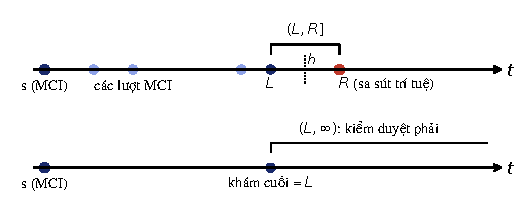
\includegraphics[width=\columnwidth]{generated/figures/fig1_interval.pdf}
\caption{Kết cục kiểm duyệt khoảng tại một mốc. Trên: khởi phát nằm trong $(L,R]$ và khoảng này vắt qua chân trời $h$ (nhóm ``khoảng vắt qua $h$'' ở Mục~\ref{sec:status}). Dưới: chưa ghi nhận sa sút trí tuệ đến lần khám cuối.}\label{fig:interval}
\end{figure}

\begin{figure}[t]
\centering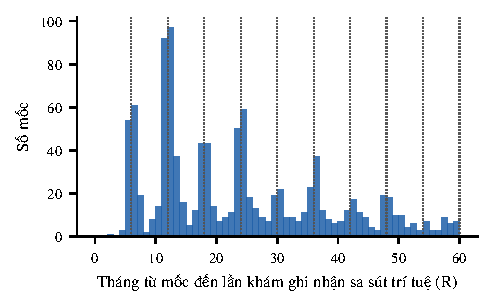
\includegraphics[width=\columnwidth]{generated/figures/fig2_heaping.pdf}
\caption{Phân bố $R$ (tháng) của các mốc có biến cố trong cửa sổ, tập train. Các cụm trùng lịch tái khám 6--12 tháng (đường chấm).}\label{fig:heaping}
\end{figure}

Hình~\ref{fig:interval} minh họa định nghĩa, và Hình~\ref{fig:heaping} cho thấy $R$ dồn tại các mốc 6, 12, 18, 24 tháng theo lịch tái khám. Đây chính là lý do phải mô hình hóa kiểm duyệt khoảng.

\subsection{Toán tử đặc trưng theo thời điểm mốc}
Với một chuỗi đo $\{(t_\ell,y_\ell)\}$ của người $i$, đặt $\ell^\star=\arg\max\{\ell: t_\ell\le s\}$ và định nghĩa toán tử ``giá trị gần nhất trong cửa sổ $\Delta$'':
\begin{equation}\label{eq:last}
\operatorname{last}_\Delta(s) = y_{\ell^\star}\quad\text{nếu } s-t_{\ell^\star}\le\Delta,
\end{equation}
và gán thiếu trong trường hợp ngược lại. Hệ thống dùng $\Delta=45$ ngày cho các thang đo nhận thức và $\Delta=365$ ngày cho MRI. Phân tích S8 dùng thêm độ trễ $\ell$: chỉ xét ảnh có $t\le s-\ell$. Chuỗi xu hướng của một thang đo gồm mọi điểm có $t\le s$, và chỉ được dùng khi trải ít nhất 300 ngày. Chuỗi MRI chỉ gồm các ảnh có cùng khóa ``phiên bản FreeSurfer $|$ cường độ từ trường'' với ảnh hiện tại (S10 thêm model máy chụp vào khóa) và phải có ICV đầy đủ. Tốc độ hai điểm (dùng trong S2a) lấy ảnh cùng chuỗi gần nhất cách ảnh hiện tại ít nhất 90 ngày.

\begin{proposition}[Đặc trưng không dùng thông tin tương lai]\label{prop:nofuture}
Với mọi mốc $(i,s)$ và mọi tham số $\bm\theta$ cố định, $\bm z_i(s)=\varphi(\mathcal F_i(s);\bm\theta)$ chỉ phụ thuộc vào dữ liệu của người $i$ có ngày $\le s$, cùng với các thuộc tính bất biến (năm sinh).
\end{proposition}
\begin{IEEEproof}
Mỗi thành phần của $\bm z$ được tính bằng một trong các toán tử sau: $\operatorname{last}_\Delta$; chuỗi lọc theo $t\le s$ (hoặc $t\le s-\ell$); $\tau$, tính từ lượt MCI đầu tiên, mà lượt này có ngày $\le s$ theo Định nghĩa~1; năm sinh. Phép hiệu chỉnh ICV và BLUP (Mục~\ref{sec:prep}) là hàm của các giá trị đó và của $\bm\theta$. Trong mã, các toán tử này là các phương thức \code{Sources.demographics\_at}, \code{clinical\_at}, \code{mri\_at} và \code{bsi\_at}. Kiểm thử \code{test\_features\_use\_only\_data\_up\_to\_the\_visit} xác nhận mọi ngày nguồn $\le s$.
\end{IEEEproof}

\section{Tiền xử lý: hiệu chỉnh ICV và mô hình hiệu ứng hỗn hợp}\label{sec:prep}
\subsection{Hiệu chỉnh thể tích theo ICV}
Thể tích hồi hải mã tỷ lệ với kích thước đầu. Hệ thống dùng phương pháp phần dư~\cite{voevodskaya2014}:
\begin{equation}\label{eq:icv}
\HVadj = \mathrm{HV} - b\bigl(\mathrm{ICV}-\overline{\mathrm{ICV}}\bigr),
\end{equation}
trong đó $b$ là hệ số góc OLS của HV theo ICV, và $\overline{\mathrm{ICV}}$ là trung bình ICV. Cả hai được ước lượng trên ảnh đầu tiên của những người luôn có chẩn đoán bình thường thuộc tập ước lượng $\mathcal A$. Nhóm bình thường được chọn để $b$ phản ánh quan hệ giải phẫu, không lẫn hiệu ứng bệnh. Trên toàn train: $b=2{,}145\times10^{-3}$, $\overline{\mathrm{ICV}}=1.445.236$~mm³, $n=846$.

\subsection{Mô hình hiệu ứng ngẫu nhiên tuyến tính}
Với một chuỗi (ADAS-Cog13, FAQ, $\HVadj$ hoặc độ dày nội khứu) của người $i$ tại các thời điểm $t_{i1}=0<\dots<t_{in_i}$ (năm, tính từ điểm đầu của chuỗi), xét mô hình~\cite{laird1982}
\begin{equation}\label{eq:lme}
\begin{gathered}
\bm y_i = \bm X_i(\bm\gamma+\bm u_i)+\bm\varepsilon_i,\qquad \bm X_i=[\bm 1, \bm t_i],\\
\bm u_i\sim\mathcal N(\bm 0,\bm D),\qquad \bm\varepsilon_i\sim\mathcal N(\bm 0,\sigma^2\bm I),
\end{gathered}
\end{equation}
với $\bm u_i\perp\bm\varepsilon_i$ và độc lập giữa các người.

\emph{Ước lượng mômen từ OLS theo từng người.} Chỉ người từng có chẩn đoán MCI, có $n_i\ge 3$ điểm và chuỗi trải $\ge 365$ ngày mới được dùng. Với mỗi người, tính và lưu sẵn
\[
\begin{gathered}
\bm M_i=(\bm X_i^\top\bm X_i)^{-1},\qquad \hat{\bm\beta}_i=\bm M_i\bm X_i^\top\bm y_i,\\
\mathrm{RSS}_i=\|\bm y_i-\bm X_i\hat{\bm\beta}_i\|^2,\qquad \nu_i=n_i-2.
\end{gathered}
\]

\begin{lemma}
Dưới mô hình~\eqref{eq:lme}, với thiết kế $\bm X_i$ cố định và có hạng đủ: $\mathbb E\hat{\bm\beta}_i=\bm\gamma$, $\operatorname{Cov}(\hat{\bm\beta}_i)=\bm D+\sigma^2\bm M_i$, và $\mathbb E\,\mathrm{RSS}_i=\sigma^2\nu_i$. Do đó, trên một tập người $\mathcal A$, các ước lượng
\begin{gather}
\hat{\bm\gamma}(\mathcal A)=\frac{1}{|\mathcal A|}\sum_{i\in\mathcal A}\hat{\bm\beta}_i,\qquad \hat\sigma^2(\mathcal A)=\frac{\sum_{i\in\mathcal A}\mathrm{RSS}_i}{\sum_{i\in\mathcal A}\nu_i},\label{eq:mom1}\\
\tilde{\bm D}(\mathcal A)=\bm S_{\hat\beta}(\mathcal A)-\hat\sigma^2(\mathcal A)\,\frac{1}{|\mathcal A|}\sum_{i\in\mathcal A}\bm M_i\label{eq:mom2}
\end{gather}
không chệch cho $\bm\gamma$, $\sigma^2$ và $\bm D$, trong đó $\bm S_{\hat\beta}$ là hiệp phương sai mẫu (mẫu số $|\mathcal A|-1$).
\end{lemma}
\begin{IEEEproof}
Ta có $\hat{\bm\beta}_i=\bm\gamma+\bm u_i+\bm M_i\bm X_i^\top\bm\varepsilon_i$. Suy ra $\mathbb E\hat{\bm\beta}_i=\bm\gamma$ và $\operatorname{Cov}\hat{\bm\beta}_i=\bm D+\sigma^2\bm M_i\bm X_i^\top\bm X_i\bm M_i=\bm D+\sigma^2\bm M_i$. Phần dư OLS là $\bm P_i^\perp\bm\varepsilon_i$ (vì $\bm P_i^\perp\bm X_i\bm u_i=\bm 0$), nên $\mathbb E\,\mathrm{RSS}_i=\sigma^2\operatorname{tr}\bm P_i^\perp=\sigma^2(n_i-2)$. Với các vector độc lập có cùng kỳ vọng và hiệp phương sai $\bm\Sigma_i$, ta có $\mathbb E\bm S=\frac{1}{|\mathcal A|}\sum_i\bm\Sigma_i$. Thay $\bm\Sigma_i=\bm D+\sigma^2\bm M_i$ và dùng tính không chệch của $\hat\sigma^2$, cùng với việc $\bm M_i$ là hằng số, thu được $\mathbb E\tilde{\bm D}=\bm D$.
\end{IEEEproof}

$\tilde{\bm D}$ có thể không xác định dương. Hệ thống chiếu nó về nón nửa xác định dương bằng cách chặn dưới trị riêng:
\begin{equation}\label{eq:psd}
\hat{\bm D}=\bm V\operatorname{diag}\bigl(\max(w_r, 10^{-6}\max(w_{\max},10^{-12}))\bigr)\bm V^\top,
\end{equation}
trong đó $\tilde{\bm D}=\bm V\operatorname{diag}(w_r)\bm V^\top$.

\begin{remark}[Chi phí ước lượng lại]
Ước lượng \eqref{eq:mom1}--\eqref{eq:mom2} chỉ cần các tổng và tổng bình phương của thống kê đã lưu sẵn. Vì vậy ước lượng lại $\bm\theta(\mathcal A)$ cho một tập $\mathcal A$ bất kỳ tốn $O(|\mathcal A|)$ phép tính và không phải khớp lại mô hình nào. Đây là điều kiện để ước lượng tham số trong từng fold, kể cả vòng lồng, trở nên khả thi (Mục~\ref{sec:design}). Trong mã: \code{Sources.\_series\_stats} lưu thống kê, \code{Sources.fit\_params} gộp chúng.
\end{remark}

\begin{lemma}[Chuỗi đã hiệu chỉnh ICV]
Gọi $\bm r_i^h,\bm r_i^c$ là phần dư OLS của HV và ICV trên cùng thiết kế $\bm X_i$. Khi đó chuỗi $\bm h_i-b(\bm c_i-\overline{\mathrm{ICV}}\bm 1)$ có hệ số OLS $\hat{\bm\beta}_i^h-b\hat{\bm\beta}_i^c+(b\,\overline{\mathrm{ICV}},0)^\top$ và
\[
\mathrm{RSS}_i^{\text{adj}}=\|\bm r_i^h\|^2-2b\langle\bm r_i^h,\bm r_i^c\rangle+b^2\|\bm r_i^c\|^2.
\]
\end{lemma}
\begin{IEEEproof}
Ước lượng OLS và phần dư đều tuyến tính theo $\bm y$, và $\bm 1$ nằm trong không gian cột của $\bm X_i$ nên phần dư của nó bằng $\bm 0$.
\end{IEEEproof}
Nhờ Bổ đề~2, chỉ cần lưu ba tích vô hướng $\|\bm r^h\|^2$, $\langle\bm r^h,\bm r^c\rangle$, $\|\bm r^c\|^2$. Từ đó thống kê của chuỗi $\HVadj$ tính được với mọi $b$, nghĩa là với mọi fold.

\subsection{BLUP của tốc độ thay đổi}
Với tham số $\hat{\bm\theta}$ cố định và chuỗi $(\bm X,\bm y)$ của người cần dự báo, chỉ gồm các điểm có $t\le s$, ta có
\begin{equation}\label{eq:blup}
\hat{\bm u}=\hat{\bm D}\bm X^\top\bm V^{-1}(\bm y-\bm X\hat{\bm\gamma}),\qquad \bm V=\bm X\hat{\bm D}\bm X^\top+\hat\sigma^2\bm I,
\end{equation}
và slope là $\hat r=\hat\gamma_1+\hat u_2$. Dưới mô hình Gauss~\eqref{eq:lme}, $\hat{\bm u}=\mathbb E[\bm u\mid\bm y]$. Đây là bộ dự báo tuyến tính không chệch có sai số bình phương trung bình nhỏ nhất (BLUP)~\cite{henderson1975,robinson1991}; khi thay tham số bằng ước lượng ta có EBLUP. BLUP co tốc độ cá nhân về $\hat\gamma_1$ theo độ tin cậy của chuỗi: chuỗi ngắn hoặc nhiễu bị co mạnh. Bảng~\ref{tab:lme} báo các tham số ước lượng trên toàn train.

\begin{table}[t]
\caption{Tham số mô hình hiệu ứng hỗn hợp (toàn train). $\gamma_0,\gamma_1$: chặn và slope trung bình (/năm); $\sqrt{D_{11}}$, $\sqrt{D_{22}}$: độ lệch chuẩn giữa người của chặn và slope; $\rho$: tương quan; $\sigma$: độ lệch chuẩn phần dư}\label{tab:lme}
\centering\footnotesize\setlength{\tabcolsep}{2.6pt}
\begin{tabular}{@{}lrrrrrrr@{}}
\toprule
Chuỗi & $n$ & $\gamma_0$ & $\gamma_1$ & $\sqrt{D_{11}}$ & $\sqrt{D_{22}}$ & $\rho$ & $\sigma$\\
\midrule
ADAS-Cog13 (điểm) & 891 & 14,3 & 1,8 & 6,3 & 2,4 & 0,48 & 3,6\\
FAQ (điểm) & 908 & 2,3 & 1,4 & 3,8 & 2,1 & 0,26 & 2,7\\
$\HVadj$ (mm³) & 790 & 6824 & $-$109 & 1055 & 130 & 0,11 & 339\\
Nội khứu (mm) & 790 & 3,070 & $-$0,0639 & 0,377 & 0,0518 & 0,27 & 0,1099\\
\bottomrule
\end{tabular}
\end{table}

\subsection{Vì sao tốc độ hai điểm không dùng được}
Với tốc độ năm hóa từ hai ảnh cách nhau $\Delta d$ ngày, $\hat r=365{,}25\,(h_2-h_1)/\Delta d$. Sai số đo độc lập cho
\begin{equation}\label{eq:var2}
\operatorname{Var}(\hat r-r)=2\sigma_m^2\Bigl(\frac{365{,}25}{\Delta d}\Bigr)^2.
\end{equation}
Độ tin cậy, tức tỷ lệ phương sai thật trên phương sai quan sát, là $\rho(\Delta d)=D_{22}/\bigl(D_{22}+\operatorname{Var}(\hat r-r)\bigr)$, với $\sqrt{D_{22}}=129{,}6$~mm³/năm (Bảng~\ref{tab:lme}). Với $\hat\sigma_m=124{,}9$~mm³ ta có:
\begin{itemize}
\item $\Delta d=206$ ngày (trung vị trên mọi mốc có cặp ảnh): độ lệch chuẩn sai số $\approx 313$~mm³/năm, $\rho=0{,}15$;
\item $\Delta d=333$ ngày (trung vị trong tập phân tích): $\approx 194$~mm³/năm, $\rho=0{,}31$.
\end{itemize}
Cả hai đều lớn hơn nhiều so với độ lớn của mức teo trung bình, $\gamma_1=-108{,}8$~mm³/năm (Hình~\ref{fig:reliability}). Đây là cơ sở lý thuyết để chọn BLUP trên chuỗi $\ge 300$ ngày làm phương pháp chính, và đưa tốc độ hai điểm vào phân tích độ nhạy S2a.

\begin{figure}[t]
\centering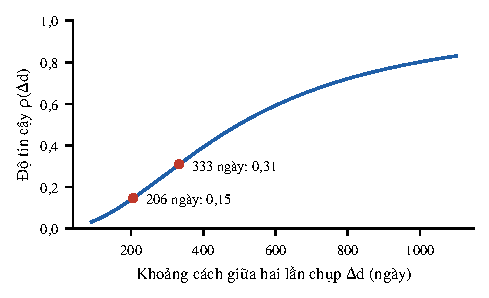
\includegraphics[width=\columnwidth]{generated/figures/fig3_reliability.pdf}
\caption{Độ tin cậy lý thuyết của tốc độ teo hồi hải mã tính từ hai ảnh, theo~\eqref{eq:var2}, với $\hat\sigma_m$ và $D_{22}$ ước lượng từ dữ liệu.}\label{fig:reliability}
\end{figure}

\section{Mô hình nguy cơ}\label{sec:model}
\subsection{Tỷ lệ nguy cơ với nguy cơ nền hằng từng khúc}
Chọn các mốc cắt $0=c_0<c_1<\dots<c_{K-1}<c_K=\infty$, gồm 6 khúc 182,5 ngày đến 1.095, 2 khúc 365 ngày đến 1.825 và một khúc mở ($K=9$). Mô hình là~\cite{cox1972,friedman1982}
\begin{gather}
\lambda(t\mid\bm z)=\alpha_{j(t)}e^{\bm\beta^\top\bm z},\qquad \alpha_j=e^{a_j},\label{eq:ph}\\
\Lambda_0(t)=\sum_{j=1}^{K}\alpha_j e_j(t),\label{eq:cumhaz}\\
e_j(t)=\min\bigl(\max(t-c_{j-1},0),\,c_j-c_{j-1}\bigr),\label{eq:exposure}\\
S(t\mid\bm z)=\exp\bigl(-\Lambda_0(t)e^{\bm\beta^\top\bm z}\bigr),\quad F(h\mid\bm z)=1-S(h\mid\bm z).\label{eq:surv}
\end{gather}
Trong đó $e_j(t)$ là thời gian nằm trong khúc $j$ trên $[0,t]$ (hàm exposure). Đặc trưng được chuẩn hóa bằng trung bình và độ lệch chuẩn của tập khớp, và các tham số này được lưu cùng mô hình. Mốc cắt đặt dày trong 3 năm đầu, nơi cần dự báo, và có thêm hai khúc đến 1.825 ngày. Nhờ vậy, khoảng $(L,R]$ vắt qua ngày 1.095 vẫn đóng góp đúng phần phơi nhiễm sau 1.095. Nếu cửa sổ chỉ đến 1.095 thì khúc cuối bị suy biến; đây là nội dung sửa đổi giao thức ghi ngày 25/11/2026.

\subsection{Hàm hợp lý có trọng số và có phạt}\label{sec:lik}
Với mốc $k$, đặt $u_k=e^{\eta_k}$, $\eta_k=\bm\beta^\top\bm z_k$, $\delta_k=\bm 1\{R_k<\infty\}$, $A_k=\Lambda_0(L_k)$ và $x_k=\bigl(\Lambda_0(R_k)-\Lambda_0(L_k)\bigr)u_k$ (với $x_k=0$ khi $\delta_k=0$). Đóng góp vào hàm hợp lý kiểm duyệt khoảng~\cite{finkelstein1986,sun2006} là
\begin{equation}\label{eq:lik}
\Pr(L_k<T_k\le R_k)=S(L_k)-S(R_k)=e^{-A_ku_k}\bigl(1-e^{-x_k}\bigr)^{\delta_k}.
\end{equation}
Một người có $n_i$ mốc; nếu coi mọi mốc là độc lập thì người có nhiều lượt khám sẽ chi phối ước lượng. Hệ thống dùng trọng số $w_k=1/n_i$ để mỗi người có tổng trọng số bằng 1, tức quần thể đích là \emph{người} chứ không phải lượt khám. Hàm mục tiêu cần tối đa hóa là
\begin{multline}\label{eq:penlik}
\ell_p(\bm a,\bm\beta)=\sum_k w_k\Bigl[-A_ku_k+\delta_k\log\bigl(1-e^{-x_k}\bigr)\Bigr]\\
-\frac{\lambda}{2}\|\bm\beta\|^2-\frac{\kappa}{2}\sum_{j=2}^{K}(a_j-a_{j-1})^2.
\end{multline}
Phạt ridge~\cite{hoerl1970} ổn định $\bm\beta$ khi các đặc trưng tương quan mạnh. Phạt sai phân bậc nhất trên log-nguy cơ là một tiên nghiệm bước ngẫu nhiên, làm trơn nguy cơ nền giữa các khúc kề nhau. Trong hệ thống $\kappa=1$; $\lambda$ được chọn từ lưới log $\{\R{lambda-grid}\}$ bằng CV lồng (Mục~\ref{sec:cv}). Vì đặc trưng đã chuẩn hóa và tổng trọng số bằng số người, $\lambda$ có thể hiểu như số ``người giả'' kéo mỗi hệ số về 0: lưới trải bốn bậc độ lớn, từ phạt không đáng kể đến phạt lớn hơn cỡ mẫu.

\subsection{Gradient giải tích}
\begin{proposition}
Đặt $\rho_k=\delta_ke^{-x_k}/(1-e^{-x_k})$. Gradient của~\eqref{eq:penlik} là
\begin{gather}
\frac{\partial\ell_p}{\partial\bm\beta}=\sum_k w_k\bigl(-A_ku_k+\rho_kx_k\bigr)\bm z_k-\lambda\bm\beta,\label{eq:gradb}\\
\frac{\partial\ell_p}{\partial a_j}=\alpha_j\sum_k w_ku_k\bigl(-e_j(L_k)+\rho_k\Delta e_{kj}\bigr)-\kappa(\bm\Delta^\top\bm\Delta\bm a)_j,\label{eq:grada}
\end{gather}
trong đó $\Delta e_{kj}=e_j(R_k)-e_j(L_k)$ và $\bm\Delta$ là ma trận sai phân bậc nhất $(K-1)\times K$.
\end{proposition}
\begin{IEEEproof}
Ta có $\partial u_k/\partial\eta_k=u_k$ và $\partial x_k/\partial\eta_k=x_k$. Từ đó $\partial(-A_ku_k)/\partial\eta_k=-A_ku_k$ và $\partial\log(1-e^{-x_k})/\partial\eta_k=\rho_kx_k$; áp dụng quy tắc dây chuyền với $\partial\eta_k/\partial\bm\beta=\bm z_k$ được~\eqref{eq:gradb}. Với $a_j$: $\partial A_k/\partial a_j=\alpha_je_j(L_k)$ và $\partial x_k/\partial a_j=\alpha_ju_k\Delta e_{kj}$, nên $\partial\log(1-e^{-x_k})/\partial a_j=\rho_k\alpha_ju_k\Delta e_{kj}$. Gradient của phạt sai phân là $\kappa\bm\Delta^\top\bm\Delta\bm a$.
\end{IEEEproof}
Hàm \code{interval\_negloglik} trả về $(-\ell_p,-\nabla\ell_p)$. Kiểm thử \code{test\_analytic\_gradient\_matches\_finite\_differences} so sánh~\eqref{eq:gradb}--\eqref{eq:grada} với sai phân trung tâm ($\varepsilon=10^{-6}$); sai số tương đối nhỏ hơn $10^{-5}$.

\subsection{Ổn định số, khởi tạo và hội tụ}
Ba biện pháp được dùng:
\begin{itemize}
\item $\log(1-e^{-x})$ được tính bằng \code{log(-expm1(-x))} với $x\ge10^{-300}$, tránh mất chữ số có nghĩa khi $x$ nhỏ;
\item $\eta$ được cắt trong $[-30,30]$ để $e^\eta$ hữu hạn;
\item khởi tạo $a_j=\log\bigl(\sum_kw_k\delta_k/\sum_kw_k\tilde t_k\bigr)$, trong đó $\tilde t_k=R_k$ nếu có biến cố và $L_k$ nếu không; khởi tạo $\bm\beta=\bm 0$.
\end{itemize}
Tối ưu bằng L-BFGS-B~\cite{byrd1995} với gradient giải tích. Hàm mục tiêu không được bảo đảm lõm đồng thời theo $(\bm a,\bm\beta)$, nên nghiệm là điểm dừng cục bộ. Hai thành phần phạt làm bài toán có điều kiện tốt hơn, và kết quả ổn định giữa các lần lặp CV. Hệ thống kiểm tra trạng thái của bộ tối ưu: thất bại cứng thì báo lỗi; dừng sớm do tìm kiếm đường (\code{ABNORMAL}) thì phát cảnh báo \code{ConvergenceWarning}. Mỗi mô hình lưu cờ \code{converged}; trên tập huấn luyện cuối cùng mọi mô hình đều hội tụ.

\begin{remark}[Khúc nguy cơ mở]
Các mốc không có biến cố bị kiểm duyệt tại $\min(L,W)\le W$. Vì vậy khúc $[1.825,\infty)$ chỉ nhận phơi nhiễm từ các khoảng có $L<W<R$ (27 khoảng trong tập ghép cặp), và ước lượng $\alpha_K$ trên khúc này lớn và không đáng tin. Khúc này không ảnh hưởng tới dự báo, vì $h\le1.095$ và $\Lambda_0(h)$ chỉ dùng $\alpha_1,\dots,\alpha_6$. Nó chỉ tác động gián tiếp qua phạt làm trơn với hệ số nhỏ $\kappa=1$. Hình~\ref{fig:baseline} vẽ $\alpha_j$ của M3 trên 8 khúc hữu hạn.
\end{remark}

\begin{figure}[t]
\centering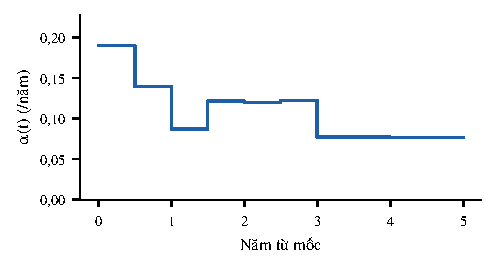
\includegraphics[width=\columnwidth]{generated/figures/fig4_baseline.pdf}
\caption{Nguy cơ nền ước lượng của M3 (tập ghép cặp, đơn vị /năm), trên 8 khúc hữu hạn.}\label{fig:baseline}
\end{figure}

\subsection{Dự báo và lấy mẫu thời điểm khởi phát có điều kiện}
Dự báo tại $h$ là $\hat F(h\mid\bm z)=-\operatorname{expm1}\bigl(-\hat\Lambda_0(h)e^{\hat{\bm\beta}^\top\bm z}\bigr)$. Đánh giá cần một thời điểm khởi phát cho các khoảng vắt qua $h$ (Mục~\ref{sec:status}). Hệ thống rút $T$ từ phân phối có điều kiện $T\mid T\in(L,R],\bm z$ theo mô hình.

\begin{proposition}
Gọi $U\sim\mathcal U(0,1)$, $\Lambda_L=\Lambda(L\mid\bm z)$, $\Lambda_R=\Lambda(R\mid\bm z)$, và đặt
\begin{equation}\label{eq:sample}
\Lambda^\star=\Lambda_L-\log\bigl(1-U\bigl(1-e^{-(\Lambda_R-\Lambda_L)}\bigr)\bigr).
\end{equation}
Khi đó $T=\Lambda^{-1}(\Lambda^\star\mid\bm z)$ có phân phối $T\mid T\in(L,R]$.
\end{proposition}
\begin{IEEEproof}
Ta có $\Pr(T\le t\mid L<T\le R)=\frac{S(L)-S(t)}{S(L)-S(R)}$. Đặt biểu thức này bằng $U$ rồi giải theo $S(t)=e^{-\Lambda(t)}$: $e^{-\Lambda(t)}=e^{-\Lambda_L}\bigl(1-U(1-e^{-(\Lambda_R-\Lambda_L)})\bigr)$, suy ra~\eqref{eq:sample}. $\Lambda_0$ tuyến tính từng khúc và đơn điệu, nên phép nghịch đảo là tìm khúc $j$ chứa $\Lambda^\star/u$ rồi nội suy tuyến tính trong khúc đó.
\end{IEEEproof}

\subsection{Mô hình Cox ridge cho quá trình kiểm duyệt}
Quá trình ngừng theo dõi được mô hình hóa bằng Cox~\cite{cox1972} có phạt ridge, xử lý mốc trùng theo Breslow~\cite{breslow1974}, có trọng số $w_k$. Thời gian là $\tilde t_k=R_k$ nếu có biến cố, ngược lại là $L_k$. ``Biến cố kiểm duyệt'' là $\delta_k^C=\bm 1\{R_k=\infty, L_k<W\}$. Các hiệp biến gồm $\tau$, tuổi, MMSE, ADAS-Cog13, FAQ. Hàm mất mát là
\begin{equation}\label{eq:cox}
\mathcal L(\bm\beta)=\sum_m d_m\log\!\!\sum_{k:\tilde t_k\ge t_m}\!\! w_ke^{\eta_k}-\sum_{k:\delta_k=1}w_k\eta_k+\frac{\lambda}{2}\|\bm\beta\|^2,
\end{equation}
với $d_m=\sum_{k:\delta_k=1,\tilde t_k=t_m}w_k$ và $\lambda=1$. Nguy cơ tích lũy nền Breslow là $\hat\Lambda_0^C(t)=\sum_{t_m\le t}d_m/\sum_{k:\tilde t_k\ge t_m}w_ke^{\hat\eta_k}$. Suy ra $\hat G(t\mid\bm z)=\exp\bigl(-\hat\Lambda_0^C(t)e^{\hat{\bm\beta}^\top\bm z}\bigr)$. Cùng lớp mô hình này, với biến cố là sa sút trí tuệ và thời điểm là ngày khám $R$, được dùng trong phân tích độ nhạy S1, tức bỏ qua kiểm duyệt khoảng.

\section{Đánh giá dưới kiểm duyệt khoảng}\label{sec:eval}
\subsection{Trạng thái tại chân trời}\label{sec:status}
Với mỗi mốc và chân trời $h$, xếp vào một trong bốn nhóm:
\begin{enumerate}
\item \emph{ca chắc chắn:} $R\le h$;
\item \emph{chắc chắn chưa:} $L\ge h$;
\item \emph{khoảng vắt qua $h$:} $L<h<R<\infty$;
\item \emph{ngừng theo dõi sớm:} $L<h$, $R=\infty$.
\end{enumerate}
Với nhóm (iii), trạng thái được quyết định bằng một thời điểm khởi phát $\tilde T$. Phân tích chính rút $\tilde T$ từ M0 theo Mệnh đề~3; M0 được chọn vì là mô hình tham chiếu trung lập, không ưu tiên mô hình nào trong cặp so sánh. Phân tích S6 thay bằng $L^+$, $(L+R)/2$, $R$, hoặc rút từ M3. Ta có $y=1$ khi ca chắc chắn hoặc $\tilde T\le h$, và $y=0$ khi chắc chắn chưa hoặc $\tilde T>h$. Hình~\ref{fig:status} cho cỡ của từng nhóm.

\begin{figure}[t]
\centering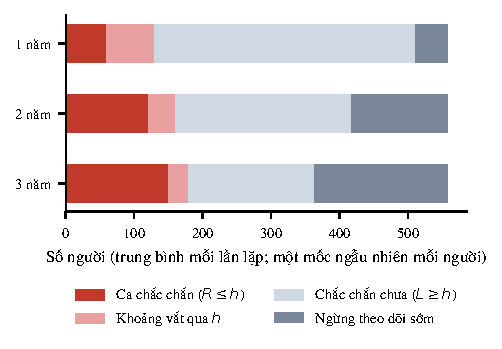
\includegraphics[width=\columnwidth]{generated/figures/fig5_status.pdf}
\caption{Bốn nhóm trạng thái tại mỗi chân trời (CV, tập ghép cặp, trung bình mỗi lần lặp). Nhóm ``ngừng theo dõi sớm'' tăng theo $h$ và được hiệu chỉnh bằng IPCW.}\label{fig:status}
\end{figure}

\subsection{Trọng số nghịch đảo xác suất kiểm duyệt}
Nhóm (iv) không có trạng thái. Nếu chỉ bỏ nhóm này thì mẫu còn lại bị chệch về phía người theo dõi lâu. Giả sử kiểm duyệt độc lập với $T$ khi biết $\bm z$. Khi đó xác suất trạng thái của một ca được quan sát là $G(R^-\mid\bm z)$, vì phải còn theo dõi tới lần khám ghi nhận, và của một người chưa có biến cố là $G(h\mid\bm z)$. Trọng số được đặt là~\cite{uno2007,gerds2006}
\begin{equation}\label{eq:ipcw}
\omega_k=\begin{cases}1/\max\{\hat G(R_k^-\mid\bm z_k),0{,}05\} & y_k=1,\\ 1/\max\{\hat G(h\mid\bm z_k),0{,}05\} & y_k=0,\\ 0 & \text{nhóm (iv)}.\end{cases}
\end{equation}
Chặn dưới 0,05 giới hạn trọng số tối đa bằng 20, đánh đổi một chút chệch lấy phương sai nhỏ hơn. Dưới giả định trên, với hàm $g$ bất kỳ, $\mathbb E[\omega\,g(y,p)]=\mathbb E[g(y,p)]$. Vì vậy các trung bình có trọng số dưới đây ước lượng không chệch (xấp xỉ, do chặn) đại lượng tương ứng khi không có kiểm duyệt.

\subsection{Phân biệt, độ chính xác tổng thể và net benefit}
Với dự báo $p_k=\hat F(h\mid\bm z_k)$, chỉ xét các mốc có $\omega_k>0$:
\begin{gather}
\mathrm{AUC}_\omega=\frac{\sum_{i:y_i=1}\sum_{j:y_j=0}\omega_i\omega_j\bigl[\bm 1(p_i>p_j)+\frac12\bm 1(p_i=p_j)\bigr]}{\sum_{i:y_i=1}\omega_i\sum_{j:y_j=0}\omega_j},\label{eq:auc}\\
\mathrm{BS}=\frac1n\sum_k\omega_k(y_k-p_k)^2,\qquad \mathrm{IPA}=1-\mathrm{BS}/\mathrm{BS}_0,\label{eq:brier}\\
\mathrm{NB}(t)=\frac{\sum_k\omega_k\bigl[y_k-(1-y_k)\frac{t}{1-t}\bigr]\bm 1(p_k\ge t)}{\sum_k\omega_k}.\label{eq:nb}
\end{gather}
$\mathrm{BS}_0$ là Brier của mô hình không hiệp biến; IPA~\cite{kattan2018} là phần cải thiện Brier so với mô hình đó, và vì là tỷ số nên không phụ thuộc cách chuẩn hóa theo $n$. Net benefit~\cite{vickers2006} quy đổi dương tính giả theo tỷ lệ cược của ngưỡng $t$, tức tỷ lệ đánh đổi lợi--hại ngầm định khi chọn ngưỡng. Đại lượng chính là $\mathrm{NB}_{\text{core}}=\frac14\sum_{t\in\{0{,}15;0{,}20;0{,}25;0{,}30\}}\mathrm{NB}(t)$, khoảng ngưỡng phù hợp với quyết định tăng cường theo dõi. Ứng dụng dùng cùng hai cận 15\% và 30\% để chia vùng nguy cơ thấp, trung bình và cao.

\subsection{Ma trận nhầm lẫn có trọng số}\label{sec:confusion}
Ứng dụng chia bệnh nhân thành ba vùng, nên người dùng cần biết một vùng có ý nghĩa gì về mặt phân loại. Với ngưỡng $t$, các ô của ma trận nhầm lẫn được tính bằng tỷ phần trọng số:
\begin{equation}\label{eq:cm}
\begin{gathered}
\mathrm{TP}(t)=\frac{\sum_k\omega_ky_k\bm 1(p_k\ge t)}{\sum_k\omega_k},\\
\mathrm{FP}(t)=\frac{\sum_k\omega_k(1-y_k)\bm 1(p_k\ge t)}{\sum_k\omega_k},
\end{gathered}
\end{equation}
và tương tự cho FN, TN; bốn ô có tổng bằng 1. Từ đó $\mathrm{Sens}=\mathrm{TP}/(\mathrm{TP}+\mathrm{FN})$, $\mathrm{Spec}=\mathrm{TN}/(\mathrm{TN}+\mathrm{FP})$, $\mathrm{PPV}=\mathrm{TP}/(\mathrm{TP}+\mathrm{FP})$, $\mathrm{NPV}=\mathrm{TN}/(\mathrm{TN}+\mathrm{FN})$ và $\mathrm{F1}=2\mathrm{TP}/(2\mathrm{TP}+\mathrm{FP}+\mathrm{FN})$. Theo cùng lập luận ở trên, các tỷ phần này ước lượng ma trận nhầm lẫn khi không có kiểm duyệt. Hệ thống tính tại hai ngưỡng của ứng dụng, $t\in\{0{,}15;0{,}30\}$, đã cố định trước khi xem kết quả. Các ô được lấy trung bình qua các lần lặp, rồi mới suy ra các tỷ số. Đây là chỉ số mô tả thứ cấp, không tham gia quy tắc quyết định. Khác với AUC, F1 phụ thuộc ngưỡng và tỷ lệ mắc tại $h$, và không dùng đến TN; vì vậy không so sánh F1 giữa các chân trời.

Mối liên hệ với net benefit giải thích cách đọc hai ngưỡng. Từ~\eqref{eq:nb} và~\eqref{eq:cm}, $\mathrm{NB}(t)=\mathrm{TP}(t)-\frac{t}{1-t}\mathrm{FP}(t)$: chọn ngưỡng $t$ tức là chấp nhận tối đa $(1-t)/t$ báo động giả cho mỗi ca được phát hiện, tương ứng 5,7 ở 15\% và 2,3 ở 30\%. Ngưỡng thấp ưu tiên bắt được ca (độ nhạy), ngưỡng cao ưu tiên độ chắc chắn khi gắn cờ (PPV). Cả hai đều nằm trong khoảng ngưỡng của $\mathrm{NB}_{\text{core}}$.

\subsection{Hiệu chuẩn bằng ước lượng Turnbull}
IPCW chỉ đúng khi mô hình kiểm duyệt đúng. Ở 730 ngày, tỷ lệ quan sát theo IPCW là \R{cv-observed-ipcw}, còn theo Turnbull là \R{cv-observed-turnbull}. Vì vậy hiệu chuẩn tuyệt đối được đánh giá bằng ước lượng không tham số cực đại hợp lý (NPMLE) của Turnbull~\cite{turnbull1976}; ước lượng này không cần mô hình kiểm duyệt.
\begin{enumerate}
\item \emph{Khoảng trong cùng:} sắp xếp mọi cận $L$ và $R$, khi trùng giá trị thì $R$ đứng trước $L$ (phù hợp với khoảng nửa mở). Các cặp liên tiếp ($L$ rồi ngay sau là $R$) tạo thành các khoảng $(q_j,p_j]$. NPMLE chỉ đặt khối xác suất trên các khoảng này.
\item \emph{Ma trận chứa:} $\alpha_{kj}=\bm 1\{q_j\ge L_k, p_j\le R_k\}$.
\item \emph{EM tự nhất quán:} lặp
\begin{equation}\label{eq:turnbull}
s_j^{(m+1)}=\frac1n\sum_k\frac{\alpha_{kj}s_j^{(m)}}{\sum_{j'}\alpha_{kj'}s_{j'}^{(m)}},
\end{equation}
cho đến khi $\max_j|s_j^{(m+1)}-s_j^{(m)}|<10^{-8}$ (tối đa 5.000 vòng).
\end{enumerate}
NPMLE chỉ xác định khối xác suất trên mỗi khoảng, không xác định cách phân bố bên trong khoảng~\cite{sun2006}. Do đó $\hat F(h)$ chỉ được kẹp giữa hai cận: $\underline F(h)=\sum_{p_j\le h}s_j$ và $\overline F(h)=\sum_{q_j<h}s_j$. Hệ thống báo trung điểm. Hiệu chuẩn được tóm tắt bằng hai đại lượng~\cite{vancalster2016}:
\begin{itemize}
\item tỷ số tổng thể $\mathrm{O/E}=\hat F_{\text{Turnbull}}(h)/\bar p$;
\item \emph{slope hiệu chuẩn nhóm:} hệ số góc OLS của $\operatorname{logit}(\hat F_g)$ theo $\operatorname{logit}(\bar p_g)$ trên 10 nhóm cùng cỡ theo hạng của $p$, với $\hat F_g$ được chặn trong $[0{,}01;0{,}99]$.
\end{itemize}
Slope nhóm là một tóm tắt mô tả trên 10 điểm tổng hợp; cách diễn giải nó được bàn ở Mục~\ref{sec:discussion}.

\section{Thiết kế kiểm định}\label{sec:design}
\subsection{CV lặp theo người với ước lượng tiền xử lý trong fold}\label{sec:cv}
Tập phân tích chính là \emph{tập ghép cặp}: các mốc có đủ mọi đầu vào của M3, gồm \R{main-landmarks} mốc của \R{main-persons} người. Trên cùng tập này, cả bốn mô hình được khớp và so sánh, nên mọi khác biệt chỉ đến từ đặc trưng. Thuật toán~\ref{alg:cv} trình bày quy trình.

\begin{algorithm}[t]
\caption{CV lặp theo người, lồng chọn $\lambda$, tiền xử lý trong fold}\label{alg:cv}
\begin{algorithmic}[1]
\Require người phân tích $\mathcal Q$, mọi người có chẩn đoán $\mathcal P$, mô hình $\{\mathcal M_m\}$, $R=20$, $F=5$, $F_{\text{in}}=3$, lưới $\Lambda$
\For{$r=1,\dots,R$}
\State chia $\mathcal Q$ ngẫu nhiên thành $F$ phần $\mathcal E_1,\dots,\mathcal E_F$ (hạt giống $42+r$)
\For{$f=1,\dots,F$}
\State $\mathcal Q_{\text{tr}}\gets\mathcal Q\setminus\mathcal E_f$; chia $\mathcal Q_{\text{tr}}$ thành $\mathcal E'_1,\dots,\mathcal E'_{F_{\text{in}}}$
\For{$g=1,\dots,F_{\text{in}}$} \Comment{vòng trong}
\State $\bm\theta\gets\bm\theta(\mathcal P\setminus\mathcal E'_g\setminus\mathcal E_f)$; tính $\bm z$
\State với mỗi $m$, $\lambda\in\Lambda$: khớp trên $\mathcal Q_{\text{tr}}\setminus\mathcal E'_g$, cộng $\ell^{w}(\lambda)$ trên $\mathcal E'_g$
\EndFor
\State $\lambda^\star_m\gets\arg\max_\lambda\sum_g\ell^{w}_g(\lambda)$
\State $\bm\theta\gets\bm\theta(\mathcal P\setminus\mathcal E_f)$; khớp $\mathcal M_m(\lambda^\star_m)$, mô hình rỗng và $\hat G$ trên $\mathcal Q_{\text{tr}}$
\State chọn ngẫu nhiên một mốc mỗi người trong $\mathcal E_f$; tính $(y,\omega)$ và $p_m$ tại $h$
\EndFor
\EndFor
\Ensure dự báo ngoài fold theo $(r,h,m)$; chỉ số theo từng lần lặp rồi lấy trung bình
\end{algorithmic}
\end{algorithm}

Điểm số của vòng trong là log-hợp lý kiểm duyệt khoảng trên phần giữ lại, không phạt, với cùng trọng số theo người $w_k=1/n_i$ như khi khớp (hàm \code{interval\_loglik}):
\begin{equation}\label{eq:innerscore}
\ell^{w}=\sum_{k\in\mathcal E'_g}w_k\Bigl[-A_ku_k+\delta_k\log\bigl(1-e^{-x_k}\bigr)\Bigr].
\end{equation}
Nhờ vậy tiêu chí chọn $\lambda$ và hàm mục tiêu~\eqref{eq:penlik} cùng nhắm tới quần thể người; ở phiên bản 7 điểm số không có trọng số, nên người có nhiều lượt khám chi phối việc chọn $\lambda$. Khi hòa, giá trị $\lambda$ đứng trước trong lưới được chọn. Mã ghi lại tỷ lệ lần chọn rơi vào hai đầu lưới và cảnh báo khi tỷ lệ này vượt 50\% (\code{edge\_share}); đây là kiểm tra trực tiếp cho lỗi của phiên bản 7. Tập ước lượng tiền xử lý $\mathcal P\setminus\mathcal E$ gồm cả những người không thuộc tập phân tích, ví dụ người luôn bình thường dùng cho~\eqref{eq:icv}, nhưng luôn loại phần đang được đánh giá.

\begin{proposition}[Không rò rỉ từ phần đánh giá]
Trong Thuật toán~\ref{alg:cv}, với mọi $i\in\mathcal E_f$, dự báo $p_m(\bm z_i(s))$ là hàm đo được của $\mathcal F_i(s)$ và của dữ liệu các người trong $\mathcal P\setminus\mathcal E_f$. Nó không phụ thuộc vào kết cục của bất kỳ người nào trong $\mathcal E_f$, cũng không phụ thuộc vào dữ liệu sau $s$ của chính $i$.
\end{proposition}
\begin{IEEEproof}
(a) $\bm\theta$ dùng để tính đặc trưng của $\mathcal E_f$ chỉ được ước lượng từ $\mathcal P\setminus\mathcal E_f$ (dòng 10). (b) $\lambda^\star$ được chọn bằng các khớp và điểm số chỉ trên $\mathcal Q_{\text{tr}}$; ở vòng trong, $\bm\theta$ còn loại thêm $\mathcal E_f$ (dòng 6). (c) Mô hình và $\hat G$ được khớp trên $\mathcal Q_{\text{tr}}$. (d) Theo Mệnh đề~\ref{prop:nofuture}, $\bm z_i(s)$ chỉ dùng $\mathcal F_i(s)$ và $\bm\theta$. Ghép (a)--(d) được kết luận. Nhãn và $\omega$ của $\mathcal E_f$ chỉ xuất hiện trong bước tính chỉ số, sau khi dự báo đã cố định.
\end{IEEEproof}

Phân tích L1 kiểm tra mức độ quan trọng của Mệnh đề~4 bằng cách ước lượng $\bm\theta$ trên toàn train (cách của các phiên bản trước). $\Delta$AUC của M3 − M2 là \R{L1-dauc-global} khi ước lượng toàn train và \R{L1-dauc-fold} khi ước lượng trong fold, tức rò rỉ có thật nhưng nhỏ.

\subsection{Một mốc mỗi người khi đánh giá}
Khi khớp, mỗi người có tổng trọng số bằng 1 (trọng số $w_k$). Khi đánh giá, mỗi người đóng góp một mốc chọn ngẫu nhiên (lặp lại ở mỗi lần lặp CV). Nhờ vậy các đơn vị đánh giá độc lập và chỉ số phản ánh hiệu năng trên người. Phân tích S3 đánh giá riêng lượt MCI thứ hai.

\subsection{Chênh lệch ghép cặp và bootstrap theo cụm người}
Với cặp $(a,b)$ và chân trời $h$, gọi $\Delta_r$ là chênh lệch (AUC, $\mathrm{NB}_{\text{core}}$, IPA) của lần lặp $r$ trên toàn bộ dự báo ngoài fold. Cả hai mô hình dùng chung $y$ và $\omega$, nên $\Delta_r$ khử phần lớn nhiễu do IPCW. Ước lượng điểm là $\bar\Delta=\frac1R\sum_r\Delta_r$. Khoảng tin cậy được tính theo Thuật toán~\ref{alg:boot}~\cite{efron1993}.

\begin{algorithm}[t]
\caption{Khoảng tin cậy bootstrap cho chênh lệch ghép cặp}\label{alg:boot}
\begin{algorithmic}[1]
\Require bảng dự báo ngoài fold theo lần lặp $\{\mathcal T_r\}$, số lần rút $B$ (1.000 cho phân tích chính, 500 cho độ nhạy)
\For{$b=1,\dots,B$}
\State rút lần lặp $r^*$ đều trong $\{1,\dots,R\}$
\State rút $n$ người có hoàn lại từ $\mathcal T_{r^*}$; tính $\Delta^{(b)}$
\EndFor
\Ensure KTC 95\% $=\bigl[Q_{0,025}(\Delta^{(b)}),\,Q_{0,975}(\Delta^{(b)})\bigr]$
\end{algorithmic}
\end{algorithm}

Khoảng này phản ánh cả biến thiên do lấy mẫu người lẫn biến thiên giữa các lần chia fold và chọn mốc. Nó không phản ánh biến thiên do khớp lại mô hình, vì dự báo được giữ cố định trong mỗi lần rút; đây là một hạn chế.

\subsection{Quy tắc quyết định khóa trước}
Với $\Delta=\mathrm{M3}-\mathrm{M2}$, gọi $[\ell_A,u_A]$ và $[\ell_N,u_N]$ là KTC 95\% của $\Delta$AUC và $\Delta\mathrm{NB}_{\text{core}}$, với $\delta=0{,}02$ và $\mu=0{,}01$:
\begin{equation}\label{eq:rule}
\text{kết luận}=\begin{cases}\text{Gia tăng} & \ell_A>0,\ \Delta\mathrm{AUC}\ge\delta,\ \ell_N>0;\\ \text{Tương đương} & -\delta<\ell_A,\ u_A<\delta,\ u_N\le\mu;\\ \text{Bất định} & \text{các trường hợp còn lại.}\end{cases}
\end{equation}
Nhánh ``tương đương'' là phiên bản khoảng tin cậy của kiểm định hai phía một chiều (TOST)~\cite{schuirmann1987}. Một KTC 95\% hai phía nằm trong $(-\delta,\delta)$ tương ứng TOST ở mức 2,5\% mỗi phía, chặt hơn mức 5\% thông thường. Nhánh ``có giá trị gia tăng'' đòi hỏi đồng thời ý nghĩa thống kê, độ lớn lâm sàng ($\ge\delta$) và lợi ích ra quyết định. Câu tổng kết chỉ được viết ``có giá trị gia tăng'' khi cả CV lẫn tập test cùng đạt nhánh đó. Toàn bộ quy tắc, cùng với $\delta$, $\mu$, các chân trời, cửa sổ, thiết kế CV và lưới $\lambda$, được khóa trong \code{config/protocol.json} trước mọi lần chạy cuối cùng. Mã đọc trực tiếp các giá trị này (Mục~\ref{sec:software}).

\emph{Sửa đổi giao thức ngày 27/11/2026.} Lưới $\lambda$ được mở rộng từ $\{0{,}1;1;10\}$ thành lưới log nửa bậc $\{\R{lambda-grid}\}$, và điểm số vòng trong chuyển sang dạng có trọng số~\eqref{eq:innerscore}. Sửa đổi này được ghi rõ là thực hiện \emph{sau} khi đã xem kết quả phiên bản 7. Lý do: ở phiên bản 7, $\lambda=10$ là cận trên của lưới và được chọn ở 372/400 lần, nên điểm tối ưu có thể nằm ngoài lưới. Trước khi chạy lại, chỉ điểm số vòng trong trên dữ liệu huấn luyện được dùng để kiểm tra rằng điểm tối ưu nằm khoảng 30--300; không chỉ số hiệu năng nào được xem. Quy tắc quyết định, các biên, chân trời, số fold và số lần lặp giữ nguyên. Ma trận nhầm lẫn (Mục~\ref{sec:confusion}) được thêm vào như chỉ số mô tả thứ cấp.

\subsection{Phân tích độ nhạy}
Mọi phân tích độ nhạy đều chạy đủ 20 lần lặp, có vòng lồng, và mang tính thăm dò. Bảng~\ref{tab:sensitivity} liệt kê chúng; trong mã, mỗi phân tích là một bản đặc tả khai báo trong \code{mci\_risk/analyses.py}.

\begin{table}[t]
\caption{Các phân tích kiểm toán và độ nhạy}\label{tab:sensitivity}
\centering\footnotesize
\begin{tabular}{@{}lL{0.8\columnwidth}@{}}
\toprule
Mã & Nội dung\\
\midrule
L1 & tham số tiền xử lý ước lượng trên toàn train (kiểm toán rò rỉ)\\
S1 & Cox chuẩn, coi ngày khám $R$ là ngày biến cố\\
S2a & tốc độ teo từ hai ảnh thay cho BLUP\\
S2b & BSI hồi hải mã~\cite{freeborough1997} (ADNI-GO/2) thay cho BLUP\\
S3 & chỉ đánh giá lượt MCI thứ hai\\
S4 & chỉ tính sa sút trí tuệ được xác nhận ở mọi lần khám sau\\
S5 & bỏ FAQ khỏi đặc trưng (cùng người với phân tích chính)\\
S6 & khởi phát tại $L^+$, $(L+R)/2$, $R$, hoặc rút từ M3\\
S7 & loại người có giới hoặc học vấn không nhất quán\\
S8 & MRI phải có trước mốc ít nhất 1, 7 hoặc 30 ngày\\
S9 & tuổi MRI: cửa sổ 180/365 ngày, hiệu năng theo tuổi ảnh, tương tác $\HVadj\times$ tuổi ảnh\\
S10 & chuỗi MRI phải cùng model máy chụp\\
\bottomrule
\end{tabular}
\end{table}

\subsection{Mô hình cuối, đánh giá test và bất định cá nhân}
Mô hình cuối có hai bộ:
\begin{itemize}
\item \emph{bộ ghép cặp:} M0--M3 khớp trên cùng tập mốc, dùng cho so sánh công bằng;
\item \emph{bộ theo dữ liệu hiện có:} mỗi mô hình khớp trên mọi mốc có đủ đầu vào của chính nó (1.176 đến 2.754 mốc). Ứng dụng dùng bộ này để dự báo cho người không có MRI lặp.
\end{itemize}
$\lambda$ của cả hai bộ được chọn bằng CV lồng 3 phần trên toàn train; với bộ ghép cặp, kết quả là \R{lambda-final}. Tập test được chấm bằng mô hình và $\bm\theta$ đã đóng băng, với 20 lần lặp chọn ngẫu nhiên một mốc mỗi người; không có gì được khớp lại.

Khoảng 95\% của nguy cơ cá nhân trong ứng dụng đến từ 200 lần bootstrap theo người. Mỗi lần rút người có hoàn lại và khớp lại mô hình với $\lambda$ cố định. Người bị rút trùng được đổi mã để mỗi bản sao giữ trọng số 1. Khoảng là phân vị 2,5--97,5\% của $\hat F(h\mid\bm z)$ qua 200 mô hình. Khoảng này bỏ qua bất định của $\bm\theta$, vì đặc trưng được tính một lần.

\section{Kiến trúc phần mềm}\label{sec:software}
\subsection{Nguyên tắc thiết kế}
Kiến trúc được dẫn dắt bởi năm yêu cầu:
\begin{itemize}
\item \emph{Một nguồn cấu hình:} mọi hằng số của giao thức chỉ được định nghĩa một lần. Nhờ vậy mã và giao thức không thể lệch nhau. Ví dụ, hai ngưỡng vùng nguy cơ của ứng dụng và hai ngưỡng của ma trận nhầm lẫn cùng lấy từ \code{BAND\_THRESHOLDS}.
\item \emph{Chiều phụ thuộc một hướng:} các script điều phối và giao diện phụ thuộc vào thư viện, không bao giờ ngược lại. Nhờ vậy các thành phần lý thuyết (Mục~\ref{sec:data}--\ref{sec:design}) kiểm thử được độc lập.
\item \emph{Hàm thuần và tất định:} mô hình là dict tuần tự hóa JSON; mọi bước ngẫu nhiên đều có hạt giống cố định. Kết quả vì vậy tái lập được từng bit.
\item \emph{Nhất quán giữa huấn luyện và sử dụng}~\cite{sculley2015}: đầu vào lúc sử dụng phải thỏa đúng các ràng buộc mà đặc trưng lúc huấn luyện thỏa.
\item \emph{Dữ liệu ở mức người tham gia không rời dự án:} sản phẩm phân phối chỉ chứa mã, mô hình và kết quả tổng hợp (Mục~\ref{sec:release}).
\end{itemize}

\subsection{Ánh xạ lý thuyết sang mã}
Bảng~\ref{tab:mapping} ánh xạ từng khái niệm lý thuyết sang module và hàm cài đặt nó; Hình~\ref{fig:architecture} cho cấu trúc phân tầng.

\begin{figure}[t]
\centering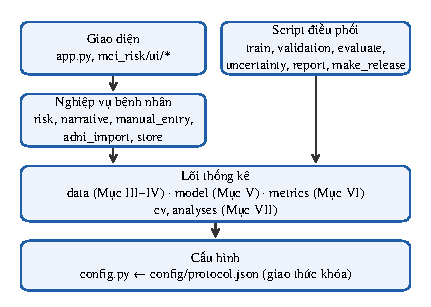
\includegraphics[width=\columnwidth]{generated/figures/fig6_architecture.pdf}
\caption{Kiến trúc phân tầng của mã nguồn v8. Mũi tên là chiều import; không có phụ thuộc ngược lên trên.}\label{fig:architecture}
\end{figure}

\begin{table}[t]
\caption{Ánh xạ lý thuyết sang mã nguồn}\label{tab:mapping}
\centering\footnotesize
\begin{tabular}{@{}L{0.40\columnwidth}L{0.55\columnwidth}@{}}
\toprule
Khái niệm & Module · hàm\\
\midrule
Mốc, khoảng $(L,R]$ \eqref{eq:interval} & \code{data}: \code{eligible\_points}, \code{attach\_labels}\\
Toán tử theo mốc (Mệnh đề~1) & \code{data}: \code{Sources.*\_at}, \code{raw\_points}\\
$\hat\sigma_m$ \eqref{eq:sigma} & \code{data}: \code{\_measurement\_error}\\
ICV, mômen, PSD \eqref{eq:icv}--\eqref{eq:psd} & \code{data}: \code{Sources.fit\_params}, \code{\_pool\_mixed\_model}\\
BLUP \eqref{eq:blup} & \code{data}: \code{blup\_slope}, \code{apply\_params}\\
Hợp lý, gradient \eqref{eq:penlik}--\eqref{eq:grada} & \code{model}: \code{interval\_negloglik}, \code{fit\_interval}\\
Lấy mẫu khởi phát \eqref{eq:sample} & \code{model}: \code{sample\_times}\\
Cox, Breslow \eqref{eq:cox} & \code{model}: \code{fit\_cox}, \code{cox\_cumhaz}\\
Trạng thái, IPCW \eqref{eq:ipcw} & \code{metrics}: \code{categories}, \code{status}\\
AUC, IPA, NB \eqref{eq:auc}--\eqref{eq:nb} & \code{metrics}: \code{summarize}, \code{net\_benefit}\\
Ma trận nhầm lẫn \eqref{eq:cm} & \code{metrics}: \code{confusion}, \code{confusion\_rates}\\
Turnbull \eqref{eq:turnbull} & \code{metrics}: \code{turnbull}, \code{turnbull\_calibration}\\
Thuật toán~1, điểm số \eqref{eq:innerscore} & \code{cv}: \code{run\_cv}, \code{lambda\_scores}, \code{interval\_loglik}, \code{edge\_share}\\
Thuật toán~2, quy tắc \eqref{eq:rule} & \code{cv}: \code{paired\_deltas}; \code{metrics}: \code{decide}\\
Bảng~\ref{tab:sensitivity} & \code{analyses}: \code{ANALYSES}\\
Dự báo cá nhân, khoảng 95\% & \code{risk}: \code{estimate}, \code{applicable\_models}\\
Vị trí trong nhóm nghiên cứu & \code{risk}: \code{risk\_distribution}, \code{share\_below}\\
Diễn giải cho từng bệnh nhân & \code{narrative}: \code{patient\_summary}, \code{comparison\_note}\\
Đóng gói không kèm dữ liệu & \code{release}: \code{release\_files}, \code{check}\\
\bottomrule
\end{tabular}
\end{table}

\subsection{Ràng buộc nhất quán khi nhập liệu thủ công}
Đặc trưng lúc huấn luyện thỏa một tập ràng buộc $\mathcal C$ do các toán tử ở Mục~\ref{sec:data} tạo ra. Vì vậy một bệnh nhân nhập tay chỉ được chấp nhận khi đầu vào của họ thỏa $\mathcal C$:
\begin{itemize}
\item mọi ngày trong lịch sử nhận thức $<s$;
\item ngày MRI $m\in[s-365,s]$;
\item mọi ảnh trong lịch sử MRI có ngày $<m$ và cùng cường độ từ trường với ảnh hiện tại;
\item ba số đo MRI phải có đủ hoặc cùng vắng;
\item mỗi giá trị nằm trong miền mà mô hình đã thấy khi huấn luyện;
\item chuỗi xu hướng trải $\ge300$ ngày, nếu không thì slope để trống.
\end{itemize}
Đầu vào vi phạm $\mathcal C$ bị từ chối kèm lý do (ngoại lệ \code{InvalidEntry}), thay vì cho ra một ước lượng nằm ngoài phân phối huấn luyện. Ứng dụng chọn mô hình đầy đủ nhất có đủ đầu vào: $\max\{m:\bm z\text{ đủ cho }\mathcal M_m\}$. M3 còn cần chuỗi MRI trải $\ge300$ ngày.

\subsection{Diễn giải kết quả trong ứng dụng}
Mỗi biểu đồ trong ứng dụng có một đoạn chú thích ngắn, viết từ chính các con số đang hiển thị. Trang nguy cơ bệnh nhân mở đầu bằng một đoạn tổng quan duy nhất cho bệnh nhân đang chọn: nguy cơ tại chân trời, khoảng 95\%, vùng nguy cơ và cận của vùng, vị trí so với nhóm nghiên cứu, các yếu tố đẩy nguy cơ lên và xuống nhiều nhất, cảnh báo khi khoảng 95\% vắt qua cận vùng, và mô hình được dùng. Phần so sánh bốn mô hình có đoạn giải thích riêng: bước thêm dữ liệu làm thay đổi ước lượng nhiều nhất, các mô hình có cùng vùng hay không, và khoảng 95\% có chồng nhau hay không. Các đoạn này được sinh bởi các hàm thuần trong \code{mci\_risk/narrative.py} và có kiểm thử riêng. Trang hiệu năng có thêm thẻ ma trận nhầm lẫn: chọn mô hình, chân trời, ngưỡng (15\% hoặc 30\%) và nguồn (CV hoặc test), hiển thị bốn ô trên 100 người có trạng thái xác định cùng Sens, Spec, PPV, NPV, F1.

\subsection{Quản trị dữ liệu và đóng gói}\label{sec:release}
Thỏa thuận sử dụng dữ liệu ADNI không cho phép phân phối lại dữ liệu. Phiên bản 7 đóng gói cả \code{data/train} và các tệp có một dòng mỗi người hoặc mỗi lượt khám (\code{train\_inputs.csv}, \code{train\_landmarks.csv}, \code{conflicts.csv}, \code{main\_oof.csv.gz}). Phiên bản 8 tách hai loại tệp:
\begin{itemize}
\item \emph{được phân phối:} mã nguồn, giao thức, mô hình đã khớp, các bootstrap của mô hình, mọi bảng kết quả tổng hợp, và phân bố nguy cơ của nhóm nghiên cứu dưới dạng phân vị và histogram (\code{cohort\_risk.json}), đủ để ứng dụng so sánh một bệnh nhân với nhóm mà không cần dữ liệu từng người;
\item \emph{chỉ lưu tại chỗ:} dữ liệu ADNI và mọi tệp ở mức người tham gia.
\end{itemize}
Script \code{make\_release.py} tạo tệp ZIP phân phối theo danh sách loại trừ trong \code{mci\_risk/release.py}. Trước khi ghi, nó quét tiêu đề mọi tệp CSV và khóa mọi tệp JSON. Nếu còn cột định danh người tham gia (\code{RID}, \code{PTID}, \code{IMAGEUID}, \ldots), script từ chối tạo gói. Ngoại lệ duy nhất là \code{data/partition.csv}: tệp này chỉ chứa số RID và phía chia, không có số đo nào, và cần để tái lập phép chia. Khi không có dữ liệu cục bộ, ứng dụng vẫn chạy đầy đủ chức năng dự báo; trang nhóm nghiên cứu và lựa chọn ``bệnh nhân ADNI'' chỉ hiện khi có dữ liệu cục bộ.

\subsection{Kiểm chứng phần mềm}
Bộ kiểm thử gồm \R{tests} kiểm thử tự động (pytest), chia thành các nhóm:
\begin{itemize}
\item hồi quy trên dữ liệu thật: mốc mới nhất chưa có nhãn, khoảng hợp lệ, không rò rỉ khi ước lượng $\bm\theta$, đặc trưng chỉ dùng dữ liệu $\le s$, một ảnh mỗi ngày;
\item đơn vị trên dữ liệu tổng hợp có tham số biết trước: gradient, khôi phục hệ số $\log 2$, đơn điệu của $\hat F$ theo $h$, mẫu khởi phát nằm trong $(L,R]$;
\item Turnbull suy biến về hàm phân phối thực nghiệm khi khoảng rất hẹp; net benefit và ma trận nhầm lẫn có trọng số tính tay; điểm số vòng trong đếm mỗi người một lần; quy tắc hòa và tỷ lệ chọn ở biên lưới $\lambda$; ba nhánh của~\eqref{eq:rule};
\item các đoạn diễn giải cho bệnh nhân; phân bố nguy cơ tổng hợp;
\item ràng buộc $\mathcal C$, kho bệnh nhân, nhập ZIP; công cụ đóng gói bỏ dữ liệu ở mức người và từ chối gói còn cột định danh;
\item tính nhất quán giữa giao thức và mã;
\item hiển thị mọi trang của ứng dụng, kể cả khi thiếu kết quả hoặc thiếu dữ liệu cục bộ.
\end{itemize}
Trước khi sửa, mã v7 được chạy lại trong môi trường mới và tái lập đúng từng tệp kết quả test của v7 (sai khác 0), nên mọi thay đổi số liệu trong bài đến từ sửa đổi giao thức chứ không từ môi trường.

\section{Kết quả}\label{sec:results}
\subsection{Mẫu nghiên cứu}
Tập ghép cặp gồm \R{main-persons} người với \R{main-landmarks} mốc (trung vị 2 mốc mỗi người). Có \R{events-persons} người có sa sút trí tuệ trong cửa sổ ở ít nhất một mốc, và \R{events-landmarks} mốc có biến cố. Trong bộ theo dữ liệu hiện có, M0--M3 có lần lượt \R{available-persons-M0}, \R{available-persons-M1}, \R{available-persons-M2} và \R{available-persons-M3} người. Trên test, \R{test-labelled-persons} người có mốc gắn nhãn (\R{test-labelled-landmarks} mốc), và tập ghép cặp có \R{test-persons} người (\R{test-landmarks} mốc). Ở 730 ngày, trung bình mỗi lần lặp CV có \R{cv-status-casecertain} ca chắc chắn, \R{cv-status-controlcertain} chắc chắn chưa, \R{cv-status-ambiguous} khoảng vắt qua và \R{cv-status-censoredearly} ngừng theo dõi sớm (Hình~\ref{fig:status}). Trong \R{lambda-choices} lần chọn $\lambda$ của CV chính, các giá trị thường gặp nhất là \R{lambda-top}; tỷ lệ lần chọn ở hai đầu lưới tối đa là \R{lambda-edge-max} cho mỗi mô hình, nên điểm tối ưu nằm trong lưới.

\subsection{Hệ số mô hình}
Bảng~\ref{tab:hr} báo tỷ số nguy cơ trên một độ lệch chuẩn của mỗi đặc trưng. Theo dõi nhận thức và chức năng (ADAS-Cog13, FAQ, RAVLT) mang phần lớn thông tin tiên lượng. Khi thêm MRI, hệ số của ADAS-Cog13 giảm, nhất quán với việc teo não và suy giảm nhận thức chia sẻ thông tin. So với phiên bản 7 ($\lambda=10$), $\lambda$ lớn hơn làm chuẩn $\|\bm\beta\|$ giảm: đa số tỷ số nguy cơ co về gần 1 (ví dụ ADAS-Cog13 trong M3 từ 1,42 xuống 1,17). Một vài hệ số của các đặc trưng tương quan với nhau, như slope ADAS-Cog13 và slope FAQ, lại tăng nhẹ, vì phạt ridge co cả vector chứ không co từng hệ số riêng lẻ. Đây là hệ số của mô hình dự báo, không mang ý nghĩa nhân quả.

\begin{table}[t]
\caption{Tỷ số nguy cơ trên 1 độ lệch chuẩn (bộ ghép cặp, $\lambda$ chọn bằng CV lồng)}\label{tab:hr}
\centering\footnotesize
\begin{tabular}{@{}lrrr@{}}
\toprule
Đặc trưng & ĐLC & HR (M0) & HR (M3)\\
\midrule
τ (năm từ MCI đầu) & 2,17 & 0,87 & 0,95\\
τ² & 20,7 & 0,93 & 0,98\\
Tuổi & 7,40 & 1,02 & 0,98\\
Giới (1 nam, 2 nữ) & 0,482 & 1,03 & 1,00\\
Học vấn & 2,82 & 1,06 & 1,03\\
MMSE & 2,24 & 0,90 & 0,92\\
FAQ & 4,34 & 1,38 & 1,17\\
ADAS-Cog13 & 7,35 & 1,43 & 1,17\\
RAVLT trì hoãn & 4,13 & 0,77 & 0,88\\
HV$_{\text{adj}}$ & 1.135 & — & 0,90\\
Độ dày nội khứu & 0,425 & — & 0,94\\
MRI 3T & 0,494 & — & 0,90\\
Slope ADAS-Cog13 & 1,34 & — & 1,16\\
Slope FAQ & 0,942 & — & 1,14\\
Slope HV$_{\text{adj}}$ & 58,3 & — & 0,94\\
Slope nội khứu & 0,0305 & — & 0,90\\
\bottomrule
\end{tabular}

\end{table}

\subsection{Hiệu năng trong CV}
Bảng~\ref{tab:cv} báo kết quả CV. Bốn mô hình đều phân biệt tốt, với AUC \R{cv-auc-range}. Hiệu chuẩn tổng thể sát: O/E Turnbull từ \R{cv-oe-range}. Slope hiệu chuẩn nhóm từ \R{cv-slope-range}; cách diễn giải đại lượng này được bàn ở Mục~\ref{sec:discussion}. Ở 730 ngày, NB(0,20) của các mô hình là \R{cv-nb20-range}, cao hơn chiến lược theo dõi tất cả (\R{cv-treatall20}). Đường quyết định (Hình~\ref{fig:decision}) nằm trên cả hai chiến lược mặc định trong toàn khoảng 5--40\%; ở ngưỡng 5\% thì gần như trùng với theo dõi tất cả, và khoảng cách tăng dần theo ngưỡng.

\begin{table}[t]
\caption{Hiệu năng CV lặp \R{cv-design} trên tập ghép cặp (\R{main-persons} người)}\label{tab:cv}
\centering\footnotesize
\begin{tabular}{@{}llrrrrrr@{}}
\toprule
$h$ & Mô hình & AUC & Brier & IPA & O/E & Slope & NB$_{\text{core}}$\\
\midrule
\multirow{4}{*}{365} & M0 & 0,866 & 0,136 & 0,259 & 1,01 & 1,77 & 0,130\\
 & M1 & 0,868 & 0,134 & 0,269 & 1,00 & 1,68 & 0,136\\
 & M2 & 0,871 & 0,134 & 0,272 & 1,01 & 1,72 & 0,134\\
 & M3 & 0,875 & 0,132 & 0,279 & 1,01 & 1,68 & 0,138\\
\midrule
\multirow{4}{*}{730} & M0 & 0,876 & 0,149 & 0,340 & 0,96 & 1,67 & 0,228\\
 & M1 & 0,886 & 0,142 & 0,371 & 0,96 & 1,60 & 0,234\\
 & M2 & 0,888 & 0,141 & 0,374 & 0,96 & 1,65 & 0,234\\
 & M3 & 0,891 & 0,139 & 0,384 & 0,96 & 1,57 & 0,236\\
\midrule
\multirow{4}{*}{1.095} & M0 & 0,874 & 0,155 & 0,382 & 0,93 & 1,79 & 0,291\\
 & M1 & 0,886 & 0,145 & 0,419 & 0,92 & 1,75 & 0,302\\
 & M2 & 0,889 & 0,145 & 0,422 & 0,92 & 1,83 & 0,301\\
 & M3 & 0,892 & 0,142 & 0,433 & 0,91 & 1,82 & 0,302\\
\bottomrule
\end{tabular}

\end{table}

\begin{figure}[t]
\centering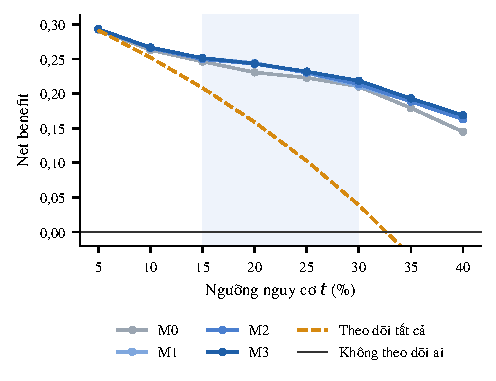
\includegraphics[width=\columnwidth]{generated/figures/fig7_decision.pdf}
\caption{Đường quyết định ở 730 ngày (CV). Vùng tô là khoảng ngưỡng dùng cho $\mathrm{NB}_{\text{core}}$.}\label{fig:decision}
\end{figure}

\subsection{Ma trận nhầm lẫn tại hai ngưỡng của ứng dụng}
Bảng~\ref{tab:confusion} báo các chỉ số phân loại ở 730 ngày trong CV. Ở ngưỡng 15\%, M3 có độ nhạy \R{cm-cv-M3-15-sensitivity} và NPV \R{cm-cv-M3-15-npv}: rất ít người sẽ được chẩn đoán bị xếp vào vùng thấp. Cái giá là độ đặc hiệu \R{cm-cv-M3-15-specificity} và PPV \R{cm-cv-M3-15-ppv}. Ở ngưỡng 30\%, độ đặc hiệu tăng lên \R{cm-cv-M3-30-specificity} và PPV lên \R{cm-cv-M3-30-ppv}, đổi lại độ nhạy giảm còn \R{cm-cv-M3-30-sensitivity}. F1 của M3 là \R{cm-cv-M3-15-f1} và \R{cm-cv-M3-30-f1} ở hai ngưỡng, so với \R{cm-cv-M2-15-f1} và \R{cm-cv-M2-30-f1} của M2; khác biệt nhỏ này nhất quán với kết quả $\Delta$AUC. Trên test, M3 ở ngưỡng 15\% có độ nhạy \R{cm-test-M3-15-sensitivity} và PPV \R{cm-test-M3-15-ppv}; ở 30\% là \R{cm-test-M3-30-sensitivity} và \R{cm-test-M3-30-ppv}. Với khoảng 30 ca ở 730 ngày, các tỷ số trên test dao động mạnh theo mẫu.

\begin{table}[t]
\caption{Chỉ số phân loại có trọng số IPCW ở 730 ngày (CV, tập ghép cặp). Gắn cờ: tỷ lệ người có nguy cơ dự báo $\geq$ ngưỡng}\label{tab:confusion}
\centering\footnotesize
\begin{tabular}{@{}llrrrrrr@{}}
\toprule
Ngưỡng & Mô hình & Sens & Spec & PPV & NPV & F1 & Gắn cờ\\
\midrule
\multirow{4}{*}{$\geq 15\%$} & M0 & 0,97 & 0,39 & 0,44 & 0,97 & 0,60 & 73\%\\
 & M1 & 0,97 & 0,46 & 0,46 & 0,96 & 0,63 & 68\%\\
 & M2 & 0,96 & 0,45 & 0,46 & 0,96 & 0,62 & 69\%\\
 & M3 & 0,96 & 0,46 & 0,47 & 0,96 & 0,63 & 68\%\\
\midrule
\multirow{4}{*}{$\geq 30\%$} & M0 & 0,80 & 0,82 & 0,69 & 0,89 & 0,74 & 38\%\\
 & M1 & 0,79 & 0,83 & 0,70 & 0,89 & 0,74 & 37\%\\
 & M2 & 0,80 & 0,83 & 0,70 & 0,90 & 0,75 & 38\%\\
 & M3 & 0,81 & 0,84 & 0,71 & 0,90 & 0,76 & 37\%\\
\bottomrule
\end{tabular}

\end{table}

\subsection{Giá trị gia tăng}
Bảng~\ref{tab:deltas} báo chênh lệch ghép cặp theo từng tầng. Ở 730 ngày trong CV, M3 − M2 có $\Delta$AUC = \R{cv-M3M2-730-dauc} \R{cv-M3M2-730-auc-ci} và $\Delta\mathrm{NB}_{\text{core}}$ = \R{cv-M3M2-730-dnb} \R{cv-M3M2-730-nb-ci}, kết luận ``\R{cv-M3M2-730-rule-lc}''; ở 1.095 ngày là ``\R{cv-M3M2-1095-rule-lc}''. Trên test, khoảng tin cậy rộng hơn và kết luận ở 365, 730 và 1.095 ngày lần lượt là ``\R{test-M3M2-365-rule-lc}'', ``\R{test-M3M2-730-rule-lc}'' và ``\R{test-M3M2-1095-rule-lc}''. Theo quy tắc báo cáo, kết luận chung là chưa đủ bằng chứng về giá trị gia tăng ổn định của tốc độ teo từ MRI lặp. Đóng góp lớn nhất đến từ một lần MRI (M1 − M0 ở 730 ngày: \R{cv-M1M0-730-dauc}; \R{cv-M1M0-730-auc-ci}), còn xu hướng nhận thức (M2 − M1) ``\R{cv-M2M1-730-rule-lc}''.

\begin{table*}[t]
\caption{Chênh lệch ghép cặp (KTC 95\% bootstrap cụm người)}\label{tab:deltas}
\centering\footnotesize
\begin{tabular}{@{}llllll@{}}
\toprule
Tầng & So sánh & $h$ & ΔAUC & ΔNB$_{\text{core}}$ & Kết luận\\
\midrule
CV & M1 − M0 & 365 & 0,002 (−0,018; 0,024) & 0,005 (−0,006; 0,016) & Bất định\\
CV & M1 − M0 & 730 & 0,010 (−0,011; 0,032) & 0,007 (−0,007; 0,020) & Bất định\\
CV & M1 − M0 & 1.095 & 0,012 (−0,008; 0,033) & 0,011 (0,000; 0,023) & Bất định\\
CV & M2 − M1 & 365 & 0,002 (−0,007; 0,011) & −0,002 (−0,008; 0,005) & Tương đương\\
CV & M2 − M1 & 730 & 0,002 (−0,007; 0,013) & 0,000 (−0,005; 0,006) & Tương đương\\
CV & M2 − M1 & 1.095 & 0,003 (−0,008; 0,013) & −0,001 (−0,010; 0,006) & Tương đương\\
CV & M3 − M2 & 365 & 0,005 (−0,003; 0,013) & 0,004 (−0,003; 0,011) & Bất định\\
CV & M3 − M2 & 730 & 0,003 (−0,006; 0,012) & 0,002 (−0,005; 0,007) & Tương đương\\
CV & M3 − M2 & 1.095 & 0,003 (−0,007; 0,013) & 0,001 (−0,006; 0,008) & Tương đương\\
\midrule
Test & M1 − M0 & 365 & −0,007 (−0,037; 0,025) & 0,001 (−0,018; 0,020) & Bất định\\
Test & M1 − M0 & 730 & 0,000 (−0,025; 0,031) & 0,000 (−0,023; 0,019) & Bất định\\
Test & M1 − M0 & 1.095 & 0,004 (−0,016; 0,029) & 0,011 (−0,005; 0,029) & Bất định\\
Test & M2 − M1 & 365 & −0,002 (−0,020; 0,016) & −0,004 (−0,021; 0,011) & Bất định\\
Test & M2 − M1 & 730 & −0,002 (−0,016; 0,012) & −0,003 (−0,014; 0,005) & Tương đương\\
Test & M2 − M1 & 1.095 & −0,002 (−0,015; 0,009) & 0,008 (−0,001; 0,017) & Bất định\\
Test & M3 − M2 & 365 & −0,006 (−0,022; 0,014) & −0,004 (−0,016; 0,009) & Bất định\\
Test & M3 − M2 & 730 & −0,004 (−0,019; 0,014) & 0,005 (−0,007; 0,020) & Bất định\\
Test & M3 − M2 & 1.095 & 0,002 (−0,009; 0,016) & −0,011 (−0,024; 0,001) & Tương đương\\
\bottomrule
\end{tabular}

\end{table*}

\subsection{Độ nhạy}
Hình~\ref{fig:forest} tóm tắt các phân tích độ nhạy ở 730 ngày; \R{sens-include-zero}/\R{sens-count} khoảng tin cậy chứa 0.
\begin{itemize}
\item \emph{S1:} bỏ qua kiểm duyệt khoảng không ảnh hưởng nhiều tới phân biệt, nhưng làm hỏng hiệu chuẩn ở chân trời ngắn. Ở 365 ngày, O/E của Cox chuẩn là \R{S1-oe-cox}, so với \R{S1-oe-interval} của mô hình kiểm duyệt khoảng; IPA là \R{S1-ipa-cox} so với \R{S1-ipa-interval}.
\item \emph{S2b:} trên nhóm ADNI-GO/2 (\R{S2b-persons} người), $\Delta$AUC của M3 − M2 là \R{S2b-dauc} \R{S2b-auc-ci}, còn BSI thay BLUP cho \R{S2b-bsi-dauc}.
\item \emph{S8:} số người còn lại khi tăng độ trễ MRI lần lượt là \R{S8-1-persons}, \R{S8-7-persons} và \R{S8-30-persons}; $\Delta$AUC lần lượt là \R{S8-1-dauc}, \R{S8-7-dauc} và \R{S8-30-dauc}.
\item \emph{S9:} cửa sổ MRI 180 ngày giữ 531 người (1.018 mốc). AUC của M3 ở nhóm ảnh 181--365 ngày tuổi (\R{S9-auc-older}) so với nhóm $\le180$ ngày (\R{S9-auc-recent}).
\end{itemize}

\begin{figure*}[t]
\centering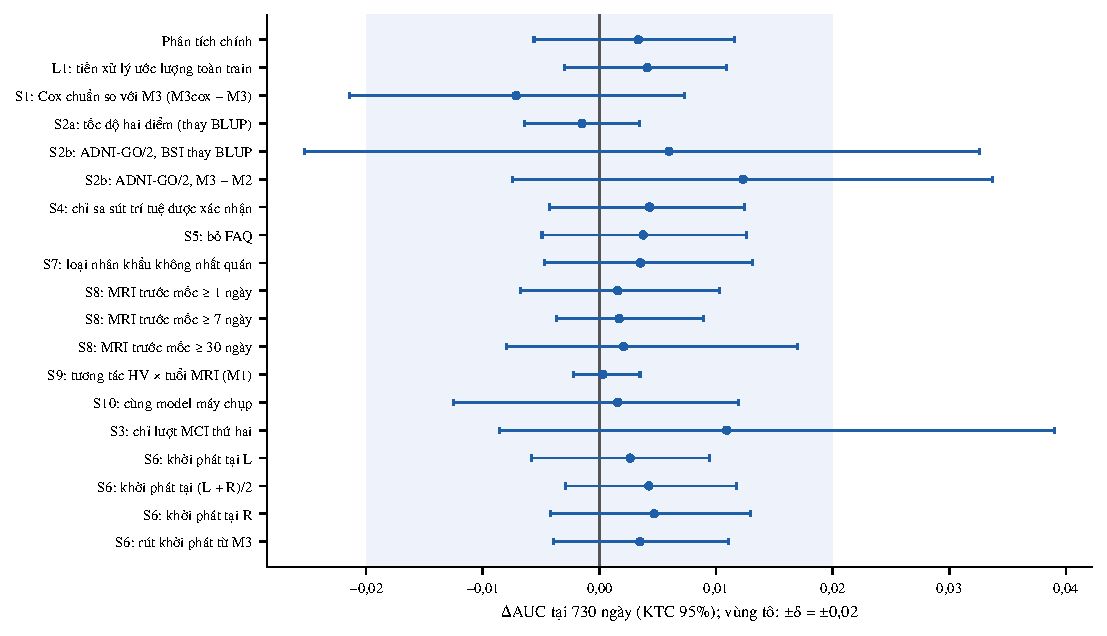
\includegraphics[width=\textwidth]{generated/figures/fig8_forest.pdf}
\caption{$\Delta$AUC ở 730 ngày trong các phân tích độ nhạy (M3 − M2, hoặc biến thay thế − M2). Vùng tô là $\pm\delta$.}\label{fig:forest}
\end{figure*}

\subsection{Tập test và bộ mô hình theo dữ liệu hiện có}
Bảng~\ref{tab:test} và Hình~\ref{fig:calibration} báo kết quả test. Ở 730 ngày, AUC đạt \R{test-auc-range} và O/E đạt \R{test-oe-range}. Slope hiệu chuẩn nhóm \R{test-slope-range} được tính trên 10 nhóm khoảng \R{test-per-group} người mỗi nhóm, nên không ổn định. Nhóm lượt MCI thứ hai trên test chỉ có 24 người, dưới ngưỡng báo cáo 60, nên không được báo.

\begin{table}[t]
\caption{Test ở 730 ngày (bộ ghép cặp) và bộ theo dữ liệu hiện có (CV và test)}\label{tab:test}
\centering\footnotesize\setlength{\tabcolsep}{3.5pt}
\begin{tabular}{@{}lrrrrrrr@{}}
\toprule
& \multicolumn{3}{c}{Test, ghép cặp} & \multicolumn{2}{c}{CV, hiện có} & \multicolumn{2}{c}{Test, hiện có}\\
\cmidrule(lr){2-4}\cmidrule(lr){5-6}\cmidrule(l){7-8}
Mô hình & AUC & O/E & Slope & Người & AUC & Người & AUC\\
\midrule
M0 & 0,925 & 1,06 & 2,42 & 865 & 0,864 & 217 & 0,877\\
M1 & 0,925 & 1,05 & 2,15 & 811 & 0,876 & 202 & 0,885\\
M2 & 0,923 & 1,06 & 2,05 & 604 & 0,889 & 151 & 0,919\\
M3 & 0,920 & 1,05 & 2,38 & 558 & 0,896 & 141 & 0,921\\
\bottomrule
\end{tabular}

\end{table}

\begin{figure}[t]
\centering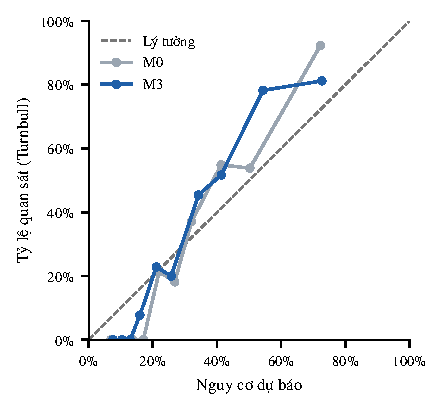
\includegraphics[width=0.8\columnwidth]{generated/figures/fig9_calibration.pdf}
\caption{Hiệu chuẩn trên test ở 730 ngày: 10 nhóm nguy cơ, tỷ lệ quan sát bằng Turnbull.}\label{fig:calibration}
\end{figure}

\section{Thảo luận}\label{sec:discussion}
\emph{Diễn giải kết quả chính.} Cả hai tầng không xác nhận giá trị gia tăng của tốc độ teo. Phân tích~\eqref{eq:var2} giải thích một phần lý do. Với khoảng cách giữa hai ảnh thường gặp, độ tin cậy của tốc độ chỉ 0,15--0,31, và BLUP chỉ có thể co chứ không thể khôi phục tín hiệu bị nhiễu che. Thêm vào đó, thể tích tại một thời điểm và độ dày nội khứu đã chứa phần lớn thông tin về quá trình teo đã xảy ra. Tín hiệu ở nhóm ADNI-GO/2 (S2b) là phân tích thăm dò trên nhóm nhỏ, không đủ để thay đổi kết luận.

\emph{Vai trò của kiểm duyệt khoảng.} S1 cho thấy mô hình hóa kiểm duyệt khoảng quyết định xác suất tuyệt đối, không quyết định thứ hạng. Cox chuẩn coi ngày khám là ngày biến cố, nên đẩy khối xác suất về phía sau trong mô hình cơ sở (trong khi biến cố thật xảy ra sớm hơn). Kết quả là dự báo ở chân trời ngắn bị lệch lớn. Với ứng dụng hiển thị xác suất cho bác sĩ, sai lệch này không chấp nhận được.

\emph{Chọn tham số phạt.} Phiên bản 7 viết rằng lưới $\lambda$ ``chưa đủ rộng về phía phạt nhỏ''. Nhận định này ngược chiều với dữ liệu: $\lambda=10$ là cận \emph{trên} của lưới và được chọn ở 372/400 lần, nên nếu điểm tối ưu nằm ngoài lưới thì nó nằm về phía phạt \emph{lớn} hơn. Thêm vào đó, điểm số vòng trong không có trọng số, không khớp với hàm mục tiêu có trọng số. Phiên bản 8 sửa cả hai điểm (Mục~\ref{sec:cv}). Với lưới mới, $\lambda$ được chọn chủ yếu trong khoảng 30--300 và không lần nào ở biên. Kết luận về giá trị gia tăng không đổi so với phiên bản 7, vì quy tắc quyết định dựa trên chênh lệch ghép cặp với cùng lưới cho mọi mô hình. Phân biệt tăng nhẹ (AUC của M3 ở 730 ngày từ 0,884 lên \R{cv-M3-730-auc}), nhưng độ chính xác tổng thể giảm nhẹ (IPA từ 0,396 xuống \R{cv-M3-730-ipa}); mục dưới giải thích lý do.

\emph{Slope hiệu chuẩn.} Trong kiểm định chéo, hệ số góc của đường hiệu chuẩn theo 10 nhóm nguy cơ nằm trong khoảng \R{cv-slope-range}. Trên thang logit, kết quả này gợi ý nguy cơ quan sát giữa các nhóm phân tán rộng hơn nguy cơ dự báo. Do hệ số được ước lượng từ 10 điểm tổng hợp và phụ thuộc vào cách chia nhóm, riêng một giá trị slope chưa đủ để kết luận mô hình bị co quá mức. Tuy vậy, hai phiên bản cho một phép so sánh trực tiếp: cùng dữ liệu, cùng fold và cùng cách chia nhóm, chỉ khác $\lambda$. Khi $\lambda$ tăng từ 10 lên 30--300, slope tăng từ 1,21--1,42 lên \R{cv-slope-range}, đồng thời IPA giảm. Như vậy phạt mạnh hơn có làm dự báo co về trung bình nhiều hơn. Tiêu chí vòng trong là log-hợp lý trên toàn cửa sổ 1.825 ngày và trên mọi lượt khám, nên nó ưu tiên mức phạt mạnh hơn mức tối ưu cho hiệu chuẩn tại các chân trời 1--3 năm. Cần phân biệt hai kết quả: khoảng trên là của CV, với khoảng \R{cv-per-group} người mỗi nhóm; trên tập test, slope là \R{test-slope-range}, nhưng mỗi nhóm chỉ khoảng \R{test-per-group} người, nên ước lượng càng kém ổn định. Một kết luận định lượng về mức co cần slope tái hiệu chuẩn ở mức cá nhân, tức khớp lại mô hình kiểm duyệt khoảng với $\hat\eta=\hat{\bm\beta}^\top\bm z$ là hiệp biến duy nhất.

\emph{Hạn chế.}
\begin{itemize}
\item Tập test nhỏ và đã được xem ở các phiên bản trước, nên chỉ là kiểm chứng nội bộ~\cite{riley2022}. Sửa đổi giao thức ngày 27/11/2026 được thực hiện sau khi đã xem kết quả phiên bản 7.
\item Nhãn sa sút trí tuệ không xác định căn nguyên; tử vong được xử lý như kiểm duyệt.
\item Giả định kiểm duyệt độc lập khi biết $\bm z$ có thể bị vi phạm nếu người suy giảm nhanh bỏ nghiên cứu.
\item Tham số hiệu ứng hỗn hợp dùng người có $\ge3$ điểm, nên có thể chệch nếu độ dài theo dõi phụ thuộc vào slope.
\item Khoảng bootstrap của $\Delta$ không phản ánh biến thiên do khớp lại mô hình; khoảng cá nhân bỏ qua bất định của $\bm\theta$.
\item Trong bảng UCSFFSX7 của tập huấn luyện, \R{qc-missing}/\R{qc-records} bản ghi (\R{qc-missing-pct}) không có giá trị ở trường \code{OVERALLQC}. Quy trình chính loại các bản ghi có cờ QC không đạt theo các tiêu chí đã mô tả và cho phép giữ bản ghi có trường QC tổng thể trống.
\item ADNI không đại diện cho quần thể Việt Nam.
\item Mô hình không dùng cho người đang điều trị kháng thể kháng amyloid.
\end{itemize}

\section{Kết luận}
Bài báo đã trình bày cơ sở lý thuyết đầy đủ của hệ thống, từ định nghĩa mốc và kết cục kiểm duyệt khoảng, qua mô hình hiệu ứng hỗn hợp, mô hình nguy cơ hằng từng khúc và khung đánh giá dưới kiểm duyệt, đến thiết kế kiểm định không rò rỉ và kiến trúc phần mềm. Mỗi thành phần có một chứng minh hoặc lập luận và một hàm cài đặt tương ứng, được kiểm thử tự động. Theo giao thức đã khóa và sửa đổi ngày 27/11/2026:
\begin{itemize}
\item trong CV, tốc độ teo từ MRI lặp ``\R{cv-M3M2-730-rule-lc}'' so với chỉ theo dõi nhận thức ở 730 ngày; trên tập test, kết quả ``\R{test-M3M2-730-rule-lc}'';
\item một lần MRI kết hợp đánh giá nhận thức và chức năng cho AUC khoảng \R{cv-M1-730-auc} ở 2 năm, với hiệu chuẩn tổng thể tốt;
\item tại ngưỡng 15\% của ứng dụng, mô hình đầy đủ nhất có độ nhạy \R{cm-cv-M3-15-sensitivity} và NPV \R{cm-cv-M3-15-npv}; tại ngưỡng 30\%, độ đặc hiệu \R{cm-cv-M3-30-specificity} và PPV \R{cm-cv-M3-30-ppv}.
\end{itemize}
Các bước tiếp theo là bổ sung amyloid, APOE, CDR và p-tau217; tính slope hiệu chuẩn ở mức cá nhân và cân nhắc chọn $\lambda$ theo tiêu chí gắn với chân trời dự báo (Brier tại $h$) trong một giao thức khóa mới; và kiểm chứng ngoài trên dữ liệu độc lập.

\appendices
\section{Tái lập kết quả}
Toàn bộ kết quả được tái lập bằng chuỗi lệnh sau, chạy trong thư mục gốc của mã nguồn, sau khi đặt dữ liệu ADNI vào \code{data/train} bằng \code{split\_dataset.py}:
\begin{enumerate}
\item \code{python -m pytest}: chạy \R{tests} kiểm thử;
\item \code{python train.py}: tham số tiền xử lý, hai bộ mô hình và phân bố nguy cơ tổng hợp;
\item \code{python validation.py}: 17 phân tích CV, khoảng 1--1,5 giờ trên 2 nhân;
\item \code{python uncertainty.py}: bootstrap cá nhân;
\item \code{python evaluate.py <thư\_mục\_test>}: chấm tập test;
\item \code{python report.py}: \code{summary.json} và bảng độ nhạy;
\item \code{python build\_report.py}: số liệu, bảng, hình, PDF và DOCX của bài này;
\item \code{python make\_release.py}: gói phân phối không kèm dữ liệu ở mức người tham gia.
\end{enumerate}
Các hạt giống ngẫu nhiên: phân fold $42+r$; chấm điểm $1042+r$; vòng trong $10r+f$; chọn $\lambda$ cuối cùng 2026; bootstrap chênh lệch 7; đánh giá test 2026; bootstrap cá nhân 42.

\section{Đối chiếu công thức với mã}
\raggedright
Với $x_k$ và $\rho_k$ như ở Mệnh đề~2, mã tính \code{one\_minus\_s = -expm1(-max(x, 1e-300))}, \code{ratio} $=\rho_k$, \code{g\_b = X.T @ (wt*(-A*u + ratio*x))} và \code{g\_a = ea*(-(EL*(wt*u)).sum(0) + (ED*(wt*ratio*u)).sum(0))}. Các biểu thức này là cài đặt trực tiếp của~\eqref{eq:gradb}--\eqref{eq:grada}, với \code{EL} $=[e_j(L_k)]$ và \code{ED} $=[\Delta e_{kj}]$. Gradient phạt: \code{g\_pen\_a[1:] += kappa*diff}, \code{g\_pen\_a[:-1] -= kappa*diff}, trong đó \code{diff} $=\Delta\bm a$; hai phép gán này cho đúng $\kappa\bm\Delta^\top\bm\Delta\bm a$. Điểm số vòng trong~\eqref{eq:innerscore} là \code{(person\_weights(frame) * contribution).sum()} trong \code{interval\_loglik}.

\begin{thebibliography}{33}
\bibitem{jack2024} C. R. Jack Jr. \emph{et al.}, ``Revised criteria for diagnosis and staging of Alzheimer's disease: Alzheimer's Association Workgroup,'' \emph{Alzheimer's Dement.}, vol. 20, no. 8, pp. 5143--5169, 2024.
\bibitem{fda2025} U.S. Food and Drug Administration, ``FDA clears first blood test used in diagnosing Alzheimer's disease,'' May 16, 2025.
\bibitem{ema} European Medicines Agency, ``Leqembi (lecanemab): product information,'' 2025.
\bibitem{belder2024} C. R. S. Belder \emph{et al.}, ``Brain volume change following anti-amyloid-$\beta$ immunotherapy for Alzheimer's disease: amyloid-removal-related pseudo-atrophy,'' \emph{Lancet Neurol.}, 2024.
\bibitem{kaufman2012} S. Kaufman, S. Rosset, C. Perlich, and O. Stitelman, ``Leakage in data mining: formulation, detection, and avoidance,'' \emph{ACM Trans. Knowl. Discov. Data}, vol. 6, no. 4, art. 15, 2012.
\bibitem{varma2006} S. Varma and R. Simon, ``Bias in error estimation when using cross-validation for model selection,'' \emph{BMC Bioinformatics}, vol. 7, art. 91, 2006.
\bibitem{tripod} G. S. Collins \emph{et al.}, ``TRIPOD+AI statement: updated guidance for reporting clinical prediction models that use regression or machine learning methods,'' \emph{BMJ}, vol. 385, e078378, 2024.
\bibitem{adni} Alzheimer's Disease Neuroimaging Initiative, ``ADNI data and documentation,'' \url{https://adni.loni.usc.edu}.
\bibitem{petersen2010} R. C. Petersen \emph{et al.}, ``Alzheimer's Disease Neuroimaging Initiative (ADNI): clinical characterization,'' \emph{Neurology}, vol. 74, no. 3, pp. 201--209, 2010.
\bibitem{fischl2012} B. Fischl, ``FreeSurfer,'' \emph{NeuroImage}, vol. 62, no. 2, pp. 774--781, 2012.
\bibitem{vanhouwelingen2007} H. C. van Houwelingen, ``Dynamic prediction by landmarking in event history analysis,'' \emph{Scand. J. Stat.}, vol. 34, no. 1, pp. 70--85, 2007.
\bibitem{voevodskaya2014} O. Voevodskaya \emph{et al.}, ``The effects of intracranial volume adjustment approaches on multiple regional MRI volumes in healthy aging and Alzheimer's disease,'' \emph{Front. Aging Neurosci.}, vol. 6, art. 264, 2014.
\bibitem{laird1982} N. M. Laird and J. H. Ware, ``Random-effects models for longitudinal data,'' \emph{Biometrics}, vol. 38, no. 4, pp. 963--974, 1982.
\bibitem{henderson1975} C. R. Henderson, ``Best linear unbiased estimation and prediction under a selection model,'' \emph{Biometrics}, vol. 31, no. 2, pp. 423--447, 1975.
\bibitem{robinson1991} G. K. Robinson, ``That BLUP is a good thing: the estimation of random effects,'' \emph{Stat. Sci.}, vol. 6, no. 1, pp. 15--32, 1991.
\bibitem{cox1972} D. R. Cox, ``Regression models and life-tables,'' \emph{J. R. Stat. Soc. B}, vol. 34, no. 2, pp. 187--202, 1972.
\bibitem{friedman1982} M. Friedman, ``Piecewise exponential models for survival data with covariates,'' \emph{Ann. Stat.}, vol. 10, no. 1, pp. 101--113, 1982.
\bibitem{finkelstein1986} D. M. Finkelstein, ``A proportional hazards model for interval-censored failure time data,'' \emph{Biometrics}, vol. 42, no. 4, pp. 845--854, 1986.
\bibitem{sun2006} J. Sun, \emph{The Statistical Analysis of Interval-censored Failure Time Data}. New York: Springer, 2006.
\bibitem{hoerl1970} A. E. Hoerl and R. W. Kennard, ``Ridge regression: biased estimation for nonorthogonal problems,'' \emph{Technometrics}, vol. 12, no. 1, pp. 55--67, 1970.
\bibitem{byrd1995} R. H. Byrd, P. Lu, J. Nocedal, and C. Zhu, ``A limited memory algorithm for bound constrained optimization,'' \emph{SIAM J. Sci. Comput.}, vol. 16, no. 5, pp. 1190--1208, 1995.
\bibitem{breslow1974} N. Breslow, ``Covariance analysis of censored survival data,'' \emph{Biometrics}, vol. 30, no. 1, pp. 89--99, 1974.
\bibitem{uno2007} H. Uno, T. Cai, L. Tian, and L. J. Wei, ``Evaluating prediction rules for $t$-year survivors with censored regression models,'' \emph{J. Amer. Statist. Assoc.}, vol. 102, no. 478, pp. 527--537, 2007.
\bibitem{gerds2006} T. A. Gerds and M. Schumacher, ``Consistent estimation of the expected Brier score in general survival models with right-censored event times,'' \emph{Biom. J.}, vol. 48, no. 6, pp. 1029--1040, 2006.
\bibitem{kattan2018} M. W. Kattan and T. A. Gerds, ``The index of prediction accuracy: an intuitive measure useful for evaluating risk prediction models,'' \emph{Diagn. Progn. Res.}, vol. 2, art. 7, 2018.
\bibitem{vickers2006} A. J. Vickers and E. B. Elkin, ``Decision curve analysis: a novel method for evaluating prediction models,'' \emph{Med. Decis. Making}, vol. 26, no. 6, pp. 565--574, 2006.
\bibitem{turnbull1976} B. W. Turnbull, ``The empirical distribution function with arbitrarily grouped, censored and truncated data,'' \emph{J. R. Stat. Soc. B}, vol. 38, no. 3, pp. 290--295, 1976.
\bibitem{vancalster2016} B. Van Calster \emph{et al.}, ``A calibration hierarchy for risk models was defined: from utopia to empirical data,'' \emph{J. Clin. Epidemiol.}, vol. 74, pp. 167--176, 2016.
\bibitem{efron1993} B. Efron and R. J. Tibshirani, \emph{An Introduction to the Bootstrap}. New York: Chapman \& Hall, 1993.
\bibitem{schuirmann1987} D. J. Schuirmann, ``A comparison of the two one-sided tests procedure and the power approach for assessing the equivalence of average bioavailability,'' \emph{J. Pharmacokinet. Biopharm.}, vol. 15, no. 6, pp. 657--680, 1987.
\bibitem{freeborough1997} P. A. Freeborough and N. C. Fox, ``The boundary shift integral: an accurate and robust measure of cerebral volume changes from registered repeat MRI,'' \emph{IEEE Trans. Med. Imag.}, vol. 16, no. 5, pp. 623--629, 1997.
\bibitem{sculley2015} D. Sculley \emph{et al.}, ``Hidden technical debt in machine learning systems,'' in \emph{Adv. Neural Inf. Process. Syst. 28}, 2015, pp. 2503--2511.
\bibitem{riley2022} R. D. Riley \emph{et al.}, ``Minimum sample size calculations for external validation of a clinical prediction model with a time-to-event outcome,'' \emph{Stat. Med.}, vol. 41, no. 7, pp. 1280--1295, 2022.
\end{thebibliography}

\end{document}
